% Options for packages loaded elsewhere
\PassOptionsToPackage{unicode}{hyperref}
\PassOptionsToPackage{hyphens}{url}
\PassOptionsToPackage{dvipsnames,svgnames*,x11names*}{xcolor}
%
\documentclass[
  12pt,
]{krantz}
\usepackage{amsmath,amssymb}
\usepackage{lmodern}
\usepackage{ifxetex,ifluatex}
\ifnum 0\ifxetex 1\fi\ifluatex 1\fi=0 % if pdftex
  \usepackage[T1]{fontenc}
  \usepackage[utf8]{inputenc}
  \usepackage{textcomp} % provide euro and other symbols
\else % if luatex or xetex
  \usepackage{unicode-math}
  \defaultfontfeatures{Scale=MatchLowercase}
  \defaultfontfeatures[\rmfamily]{Ligatures=TeX,Scale=1}
\fi
% Use upquote if available, for straight quotes in verbatim environments
\IfFileExists{upquote.sty}{\usepackage{upquote}}{}
\IfFileExists{microtype.sty}{% use microtype if available
  \usepackage[]{microtype}
  \UseMicrotypeSet[protrusion]{basicmath} % disable protrusion for tt fonts
}{}
\makeatletter
\@ifundefined{KOMAClassName}{% if non-KOMA class
  \IfFileExists{parskip.sty}{%
    \usepackage{parskip}
  }{% else
    \setlength{\parindent}{0pt}
    \setlength{\parskip}{6pt plus 2pt minus 1pt}}
}{% if KOMA class
  \KOMAoptions{parskip=half}}
\makeatother
\usepackage{xcolor}
\IfFileExists{xurl.sty}{\usepackage{xurl}}{} % add URL line breaks if available
\IfFileExists{bookmark.sty}{\usepackage{bookmark}}{\usepackage{hyperref}}
\hypersetup{
  pdftitle={Bayesian Analysis of Capture-Recapture Data with Hidden Markov Models},
  pdfauthor={Olivier Gimenez},
  colorlinks=true,
  linkcolor=Maroon,
  filecolor=Maroon,
  citecolor=Blue,
  urlcolor=Blue,
  pdfcreator={LaTeX via pandoc}}
\urlstyle{same} % disable monospaced font for URLs
\usepackage{color}
\usepackage{fancyvrb}
\newcommand{\VerbBar}{|}
\newcommand{\VERB}{\Verb[commandchars=\\\{\}]}
\DefineVerbatimEnvironment{Highlighting}{Verbatim}{commandchars=\\\{\}}
% Add ',fontsize=\small' for more characters per line
\usepackage{framed}
\definecolor{shadecolor}{RGB}{248,248,248}
\newenvironment{Shaded}{\begin{snugshade}}{\end{snugshade}}
\newcommand{\AlertTok}[1]{\textcolor[rgb]{0.94,0.16,0.16}{#1}}
\newcommand{\AnnotationTok}[1]{\textcolor[rgb]{0.56,0.35,0.01}{\textbf{\textit{#1}}}}
\newcommand{\AttributeTok}[1]{\textcolor[rgb]{0.77,0.63,0.00}{#1}}
\newcommand{\BaseNTok}[1]{\textcolor[rgb]{0.00,0.00,0.81}{#1}}
\newcommand{\BuiltInTok}[1]{#1}
\newcommand{\CharTok}[1]{\textcolor[rgb]{0.31,0.60,0.02}{#1}}
\newcommand{\CommentTok}[1]{\textcolor[rgb]{0.56,0.35,0.01}{\textit{#1}}}
\newcommand{\CommentVarTok}[1]{\textcolor[rgb]{0.56,0.35,0.01}{\textbf{\textit{#1}}}}
\newcommand{\ConstantTok}[1]{\textcolor[rgb]{0.00,0.00,0.00}{#1}}
\newcommand{\ControlFlowTok}[1]{\textcolor[rgb]{0.13,0.29,0.53}{\textbf{#1}}}
\newcommand{\DataTypeTok}[1]{\textcolor[rgb]{0.13,0.29,0.53}{#1}}
\newcommand{\DecValTok}[1]{\textcolor[rgb]{0.00,0.00,0.81}{#1}}
\newcommand{\DocumentationTok}[1]{\textcolor[rgb]{0.56,0.35,0.01}{\textbf{\textit{#1}}}}
\newcommand{\ErrorTok}[1]{\textcolor[rgb]{0.64,0.00,0.00}{\textbf{#1}}}
\newcommand{\ExtensionTok}[1]{#1}
\newcommand{\FloatTok}[1]{\textcolor[rgb]{0.00,0.00,0.81}{#1}}
\newcommand{\FunctionTok}[1]{\textcolor[rgb]{0.00,0.00,0.00}{#1}}
\newcommand{\ImportTok}[1]{#1}
\newcommand{\InformationTok}[1]{\textcolor[rgb]{0.56,0.35,0.01}{\textbf{\textit{#1}}}}
\newcommand{\KeywordTok}[1]{\textcolor[rgb]{0.13,0.29,0.53}{\textbf{#1}}}
\newcommand{\NormalTok}[1]{#1}
\newcommand{\OperatorTok}[1]{\textcolor[rgb]{0.81,0.36,0.00}{\textbf{#1}}}
\newcommand{\OtherTok}[1]{\textcolor[rgb]{0.56,0.35,0.01}{#1}}
\newcommand{\PreprocessorTok}[1]{\textcolor[rgb]{0.56,0.35,0.01}{\textit{#1}}}
\newcommand{\RegionMarkerTok}[1]{#1}
\newcommand{\SpecialCharTok}[1]{\textcolor[rgb]{0.00,0.00,0.00}{#1}}
\newcommand{\SpecialStringTok}[1]{\textcolor[rgb]{0.31,0.60,0.02}{#1}}
\newcommand{\StringTok}[1]{\textcolor[rgb]{0.31,0.60,0.02}{#1}}
\newcommand{\VariableTok}[1]{\textcolor[rgb]{0.00,0.00,0.00}{#1}}
\newcommand{\VerbatimStringTok}[1]{\textcolor[rgb]{0.31,0.60,0.02}{#1}}
\newcommand{\WarningTok}[1]{\textcolor[rgb]{0.56,0.35,0.01}{\textbf{\textit{#1}}}}
\usepackage{longtable,booktabs,array}
\usepackage{calc} % for calculating minipage widths
% Correct order of tables after \paragraph or \subparagraph
\usepackage{etoolbox}
\makeatletter
\patchcmd\longtable{\par}{\if@noskipsec\mbox{}\fi\par}{}{}
\makeatother
% Allow footnotes in longtable head/foot
\IfFileExists{footnotehyper.sty}{\usepackage{footnotehyper}}{\usepackage{footnote}}
\makesavenoteenv{longtable}
\usepackage{graphicx}
\makeatletter
\def\maxwidth{\ifdim\Gin@nat@width>\linewidth\linewidth\else\Gin@nat@width\fi}
\def\maxheight{\ifdim\Gin@nat@height>\textheight\textheight\else\Gin@nat@height\fi}
\makeatother
% Scale images if necessary, so that they will not overflow the page
% margins by default, and it is still possible to overwrite the defaults
% using explicit options in \includegraphics[width, height, ...]{}
\setkeys{Gin}{width=\maxwidth,height=\maxheight,keepaspectratio}
% Set default figure placement to htbp
\makeatletter
\def\fps@figure{htbp}
\makeatother
\setlength{\emergencystretch}{3em} % prevent overfull lines
\providecommand{\tightlist}{%
  \setlength{\itemsep}{0pt}\setlength{\parskip}{0pt}}
\setcounter{secnumdepth}{5}
\usepackage{booktabs}
\usepackage{longtable}
\usepackage[bf,singlelinecheck=off]{caption}

\usepackage{Alegreya}
\usepackage[scale=.7]{sourcecodepro}

\usepackage{framed,color}
\definecolor{shadecolor}{RGB}{248,248,248}

\renewcommand{\textfraction}{0.05}
\renewcommand{\topfraction}{0.8}
\renewcommand{\bottomfraction}{0.8}
\renewcommand{\floatpagefraction}{0.75}

\renewenvironment{quote}{\begin{VF}}{\end{VF}}
\let\oldhref\href
\renewcommand{\href}[2]{#2\footnote{\url{#1}}}

\ifxetex
  \usepackage{letltxmacro}
  \setlength{\XeTeXLinkMargin}{1pt}
  \LetLtxMacro\SavedIncludeGraphics\includegraphics
  \def\includegraphics#1#{% #1 catches optional stuff (star/opt. arg.)
    \IncludeGraphicsAux{#1}%
  }%
  \newcommand*{\IncludeGraphicsAux}[2]{%
    \XeTeXLinkBox{%
      \SavedIncludeGraphics#1{#2}%
    }%
  }%
\fi

\makeatletter
\newenvironment{kframe}{%
\medskip{}
\setlength{\fboxsep}{.8em}
 \def\at@end@of@kframe{}%
 \ifinner\ifhmode%
  \def\at@end@of@kframe{\end{minipage}}%
  \begin{minipage}{\columnwidth}%
 \fi\fi%
 \def\FrameCommand##1{\hskip\@totalleftmargin \hskip-\fboxsep
 \colorbox{shadecolor}{##1}\hskip-\fboxsep
     % There is no \\@totalrightmargin, so:
     \hskip-\linewidth \hskip-\@totalleftmargin \hskip\columnwidth}%
 \MakeFramed {\advance\hsize-\width
   \@totalleftmargin\z@ \linewidth\hsize
   \@setminipage}}%
 {\par\unskip\endMakeFramed%
 \at@end@of@kframe}
\makeatother

\makeatletter
\@ifundefined{Shaded}{
}{\renewenvironment{Shaded}{\begin{kframe}}{\end{kframe}}}
\makeatother

\newenvironment{rmdblock}[1]
  {
  \begin{itemize}
  \renewcommand{\labelitemi}{
    \raisebox{-.7\height}[0pt][0pt]{
      {\setkeys{Gin}{width=3em,keepaspectratio}\includegraphics{images/#1}}
    }
  }
  \setlength{\fboxsep}{1em}
  \begin{kframe}
  \item
  }
  {
  \end{kframe}
  \end{itemize}
  }
\newenvironment{rmdnote}
  {\begin{rmdblock}{note}}
  {\end{rmdblock}}
\newenvironment{rmdcaution}
  {\begin{rmdblock}{caution}}
  {\end{rmdblock}}
\newenvironment{rmdimportant}
  {\begin{rmdblock}{important}}
  {\end{rmdblock}}
\newenvironment{rmdtip}
  {\begin{rmdblock}{tip}}
  {\end{rmdblock}}
\newenvironment{rmdwarning}
  {\begin{rmdblock}{warning}}
  {\end{rmdblock}}

\usepackage{makeidx}
\makeindex

\urlstyle{tt}

\usepackage{amsthm}
\makeatletter
\def\thm@space@setup{%
  \thm@preskip=8pt plus 2pt minus 4pt
  \thm@postskip=\thm@preskip
}
\makeatother

\frontmatter
\usepackage{tikz}
\usepackage{pgfplots}
\usepackage{blkarray}
\ifluatex
  \usepackage{selnolig}  % disable illegal ligatures
\fi
\usepackage[]{natbib}
\bibliographystyle{plainnat}

\title{Bayesian Analysis of Capture-Recapture Data with Hidden Markov Models}
\usepackage{etoolbox}
\makeatletter
\providecommand{\subtitle}[1]{% add subtitle to \maketitle
  \apptocmd{\@title}{\par {\large #1 \par}}{}{}
}
\makeatother
\subtitle{Theory and Case Studies in R}
\author{Olivier Gimenez}
\date{2022-01-20}

\begin{document}
\maketitle

%\cleardoublepage\newpage\thispagestyle{empty}\null
%\cleardoublepage\newpage\thispagestyle{empty}\null
%\cleardoublepage\newpage
\thispagestyle{empty}

\setlength{\abovedisplayskip}{-5pt}
\setlength{\abovedisplayshortskip}{-5pt}

{
\hypersetup{linkcolor=}
\setcounter{tocdepth}{2}
\tableofcontents
}
\listoftables
\listoffigures
\hypertarget{welcome}{%
\chapter*{Welcome}\label{welcome}}


Welcome to the online version of the book \emph{Bayesian Analysis of Capture-Recapture Data with Hidden Markov Models -- Theory and Case Studies in R}.

The HMM framework has gained much attention in the ecological literature over the last decade, and has been suggested as a general modelling framework for the demography of plant and animal populations. In particular, HMMs are increasingly used to analyse capture-recapture data and estimate key population parameters (e.g., survival, dispersal, recruitment or abundance) with applications in all fields of ecology.

In parallel, Bayesian statistics is well established and fast growing in ecology and related disciplines, because it resonates with scientific reasoning and allows accommodating uncertainty smoothly. The popularity of Bayesian statistics also comes from the availability of free pieces of software (WinBUGS, OpenBUGS, JAGS, Stan, NIMBLE) that allow practitioners to code their own analyses.

This book offers a Bayesian treatment of HMMs applied to capture-recapture data. You will learn to use the R package NIMBLE which is seen by many as the future of Bayesian statistical ecology to deal with complex models and/or big data. An important part of the book consists in case studies presented in a tutorial style to abide by the ``learning by doing'' philosophy.

I'm currently writing this book, and I welcome any feedback. You may raise an issue \href{https://github.com/oliviergimenez/banana-book/issues}{here}, amend directly the R Markdown file that generated the page you're reading by clicking on the `Edit this page' icon in the right panel, or \href{mailto:olivier.gimenez@cefe.cnrs.fr}{email me}. Many thanks!

Olivier Gimenez, Montpellier, France\\
Last updated: January 20, 2022

\hypertarget{license}{%
\section*{License}\label{license}}


The online version of this book is licensed under the \href{http://creativecommons.org/licenses/by-nc-nd/4.0/}{Creative Commons Attribution-NonCommercial-NoDerivatives 4.0 International License}.

The code is public domain, licensed under \href{https://creativecommons.org/publicdomain/zero/1.0/}{Creative Commons CC0 1.0 Universal (CC0 1.0)}.

\hypertarget{preface}{%
\chapter*{Preface}\label{preface}}


\hypertarget{why-this-book}{%
\section*{Why this book?}\label{why-this-book}}


\textbf{To be completed.} Why and what of capture-recapture data and models, with fields of application.\footnote{Watch out nice Johnny Ball's video \url{https://www.youtube.com/watch?v=tyX79mPm2xY}.} Brief history of capture-recapture, with switch to state-space/hidden Markov model (HMM) formulation. Flexibility of HMM to decompose complex problems in smaller pieces that are easier to understand, model and analyse. From satellite guidance to conservation of endangered species. Why Bayes? Also three of my fav research topics -- capture-recapture, HMM and Bayes statistics -- let's enjoy this great cocktail together.

\hypertarget{who-should-read-this-book}{%
\section*{Who should read this book?}\label{who-should-read-this-book}}


This book is aimed at beginners who're comfortable using R and write basic code (including loops), as well as connoisseurs of capture-recapture who'd like to tap into the power of the Bayesian side of statistics. For both audiences, thinking in the HMM framework will help you in confidently building models and make the most of your capture-recapture data.

\hypertarget{what-will-you-learn}{%
\section*{What will you learn?}\label{what-will-you-learn}}


The book is divided into five parts. The first part is aimed at getting you up-to-speed with Bayesian statistics, NIMBLE, and hidden Markov models. The second part will teach you all about capture-recapture models for open populations, with reproducible R code to ease the learning process. In the third part, we will focus on issues in inferring states (dealing with uncertainty in assignment, modelling waiting time distribution). The fourth part provides real-world case studies from the scientific literature that you can reproduce using material covered in previous chapters. These problems can either i) be used to cement and deepen your understanding of methods and models, ii) be adapted for your own purpose, or iii) serve as teaching projects. The fifth and last chapter closes the book with take-home messages and recommendations, a list of frequently asked questions and references cited in the book. \textbf{Likely to be amended after feedbacks.}

\hypertarget{what-wont-you-learn}{%
\section*{What won't you learn?}\label{what-wont-you-learn}}


There is hardly any maths in this book. The equations I use are either simple enough to be understood without a background in maths, or can be skipped without prejudice. I do not cover Bayesian statistics or even hidden Markov models fully, I provide just what you need to work with capture-recapture data. If you are interested in knowing more about these topics, hopefully the section Suggested reading at the end of each chapter will put you in the right direction. There are also a number of important topics specific to capture-recapture that I do not cover, including closed-population capture-recapture models \citep{WilliamsEtAl2002}, and spatial capture-recapture models \citep{RoyleEtAl2013book}. These models can be treated as HMMs, but for now the usual formulation is just fine. \textbf{There will be spatial considerations in the Covariates chapter w/ splines and CAR. I'm not sure yet about SCR models (R. Glennie's Biometrics paper on HMMs and open pop SCR will not be easy to Bayes transform and implement in NIMBLE).}

\hypertarget{prerequisites}{%
\section*{Prerequisites}\label{prerequisites}}


This book uses primarily the R package NIMBLE, so you need to install at least R and NIMBLE. A bunch of other R packages are used. You can install them all at once by running:

\begin{Shaded}
\begin{Highlighting}[]
\FunctionTok{install.packages}\NormalTok{(}\FunctionTok{c}\NormalTok{(}
  \StringTok{"magick"}\NormalTok{, }\StringTok{"MCMCvis"}\NormalTok{, }\StringTok{"nimble"}\NormalTok{, }\StringTok{"pdftools"}\NormalTok{, }
  \StringTok{"tidyverse"}\NormalTok{, }\StringTok{"wesanderson"} 
\NormalTok{))}
\end{Highlighting}
\end{Shaded}

\hypertarget{acknowledgements}{%
\section*{Acknowledgements}\label{acknowledgements}}


\textbf{To be completed.}

\hypertarget{how-this-book-was-written}{%
\section*{How this book was written}\label{how-this-book-was-written}}


I am writing this book in \href{http://www.rstudio.com/ide/}{RStudio} using \href{http://bookdown.org/}{bookdown}. The \href{https://oliviergimenez.github.io/banana-book}{book website} is hosted with \href{https://pages.github.com/}{GitHub Pages}, and automatically updated after every push by \href{https://github.com/features/actions}{Github Actions}. The source is available from \href{https://github.com/oliviergimenez/banana-book}{GitHub}.

The version of the book you're reading was built with R version 4.1.0 (2021-05-18) and the following packages:

\begin{longtable}[]{@{}lll@{}}
\toprule
package & version & source \\
\midrule
\endhead
magick & 2.7.3 & CRAN (R 4.1.0) \\
MCMCvis & 0.15.3 & CRAN (R 4.1.0) \\
nimble & 0.11.1 & CRAN (R 4.1.0) \\
pdftools & 3.0.1 & CRAN (R 4.1.0) \\
tidyverse & 1.3.1 & CRAN (R 4.1.0) \\
wesanderson & 0.3.6 & CRAN (R 4.1.0) \\
\bottomrule
\end{longtable}

\hypertarget{about-the-author}{%
\chapter*{About the author}\label{about-the-author}}


My name is Olivier Gimenez (\url{https://oliviergimenez.github.io/}). I am a senior (euphemism for not so young anymore) scientist at the National Centre for Scientific Research (CNRS) in the beautiful city of Montpellier, France.

I struggled studying maths, obtained a PhD in applied statistics a long time ago in a galaxy of wine and cheese. I was awarded my habilitation (\url{https://en.wikipedia.org/wiki/Habilitation}) in ecology and evolution so that I could stop pretending to understand what my colleagues were talking about. More recently I embarked in sociology studies because hey, why not.

Lost somewhere at the interface of animal ecology, statistical modeling and social sciences, my so-called expertise lies in population dynamics and species distribution modeling to address questions in ecology and conservation biology about the impact of human activities and the management of large carnivores. I would be nothing without the students and colleagues who are kind enough to bear with me.

You may find me on Twitter (\url{https://twitter.com/oaggimenez}), GitHub (\url{https://github.com/oliviergimenez}), or get in touch \href{mailto:olivier.gimenez@cefe.cnrs.fr}{by email}.

\mainmatter

\hypertarget{part-i.-fundations}{%
\part{I. Fundations}\label{part-i.-fundations}}

\hypertarget{introduction}{%
\chapter*{Introduction}\label{introduction}}


\hypertarget{crashcourse}{%
\chapter{Bayesian statistics \& MCMC}\label{crashcourse}}

\hypertarget{introduction-1}{%
\section{Introduction}\label{introduction-1}}

In this first chapter, you will learn what the Bayesian theory is, and how you may use it with a simple example. You will also see how to implement simulation algorithms to implement the Bayesian method for more complex analyses. This is not an exhaustive treatment of Bayesian statistics, but you should get what you need to navigate through the rest of the book.

\hypertarget{bayes-theorem}{%
\section{Bayes' theorem}\label{bayes-theorem}}

Let's not wait any longer and jump into it. Bayesian statistics relies on the Bayes' theorem (or law, or rule, whatever you prefer) named after Reverend Thomas Bayes (Figure \ref{fig:revbayes}). This theorem was published in 1763 two years after Bayes' death thanks to his friend's efforts Richard Price, and was independently discovered by Pierre-Simon Laplace \citep{mcgrayne2011}.

\begin{figure}

{\centering 
\includegraphics[width=1\linewidth]{images/amazing-thomas-bayes-illustration} 

}

\caption{Cartoon of Thomas Bayes with Bayes' theorem in background. Source: [James Kulich](https://www.elmhurst.edu/blog/thomas-bayes/)}\label{fig:revbayes}
\end{figure}

As we will see in a minute, Bayes' theorem is all about conditional probabilities, which are somehow tricky to understand. Conditional probability of outcome or event A given event B, which we denote \(\Pr(A \mid B)\), is the probability that A occurs, revised by considering the additional information that event B has occurred.\footnote{For example, a friend of yours rolls a fair dice and asks you the probability that the outcome was a six (event A). Your answer is 1/6 because each side of the dice is equally likely to come up. Now imagine that you're told the number rolled was even (event B) before you answer your friend's question. Because there are only three even numbers, one of which is six, you may revise your answer for the probability that a six was rolled from 1/6 to \(\Pr(A \mid B) = 1/3\).} The order in which A and B appear is important, make sure you do not confuse \(\Pr(A \mid B)\) and \(\Pr(B \mid A)\).

Bayes' theorem (Figure \ref{fig:bayestheorem}) gives you \(\Pr(A \mid B)\) using marginal probabilities \(\Pr(A)\) and \(\Pr(B)\) and \(\Pr(B \mid A)\):
\[\Pr(A \mid B) = \displaystyle{\frac{ \Pr(B \mid A) \; \Pr(A)}{\Pr(B)}}.\]
Originally, Bayes' theorem was seen as a way to infer an unkown cause A of a particular effect B, knowing the probability of effect B given cause A. Think for example of a situation where a medical diagnosis is needed, with A an unkown disease and B symptoms, the doctor knows P(symptoms\textbar disease) and wants to derive P(disease\textbar symptoms). This way of reversing \(\Pr(B \mid A)\) into \(\Pr(A \mid B)\) explains why Bayesian thinking used to be referred to as `inverse probability'.

\textbackslash begin\{figure\}

\{\centering 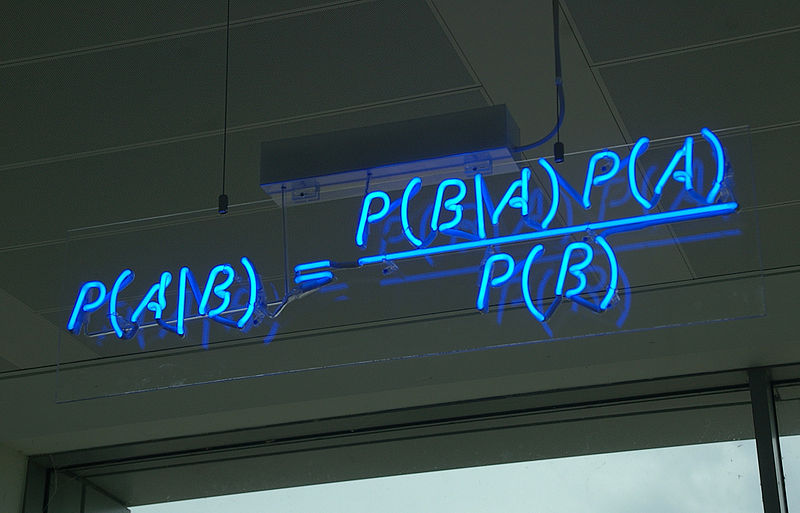
\includegraphics[width=11.11in]{images/bayes_neon}

\}

\textbackslash caption\{Bayes' theorem spelt out in blue neon. Source: \href{https://en.wikipedia.org/wiki/Bayes\%27_theorem}{Wikipedia}\}\label{fig:bayestheorem}
\textbackslash end\{figure\}

I don't know about you, but I need to think twice for not messing the letters around. I find it easier to remember Bayes' theorem written like this\footnote{When teaching Bayes' theorem, I am very much inspired by Tristan Mahr's slides from his introduction to Bayesian regression \url{https://www.tjmahr.com/bayes-intro-lecture-slides-2017/}}:

\[ \Pr(\text{hypothesis} \mid \text{data}) = \frac{ \Pr(\text{data} \mid \text{hypothesis}) \; \Pr(\text{hypothesis})}{\Pr(\text{data})} \]
\begin{rmdnote}
The \emph{hypothesis} is a working assumption about which you want to learn using \emph{data}. In capture--recapture analyses, the hypothesis might be a parameter like detection probability, or regression parameters in a relationship between survival probability and a covariate. Bayes' theorem tells us how to obtain the probability of a hypothesis given the data we have.
\end{rmdnote}

This is great because think about it, this is exactly what the scientific method is! We'd like to know how plausible some hypothesis is based on some data we collected, and possibly compare several hypotheses among them. In that respect, the Bayesian reasoning matches the scientific reasoning, which probably explains why the Bayesian framework is so natural for doing and understanding statistics.

You might ask then, why is Bayesian statistics not the default in statistics? Clearly, because of futile wars between male statisticians (including Ronald Fisher, Jerzy Neyman and Egon Sharpe Pearson among others), little progress was made for over two centuries. Also, until recently, there were practical problems to implement Bayes' theorem. Recent advances in computational power coupled with the development of new algorithms have led to a great increase in the application of Bayesian methods within the last three decades.

\hypertarget{what-is-the-bayesian-approach}{%
\section{What is the Bayesian approach?}\label{what-is-the-bayesian-approach}}

Typical statistical problems involve estimating a parameter (or several parameters) \(\theta\) with available data. To do so, you might be more used to the frequentist rather than the Bayesian method. The frequentist approach, and in particular maximum likelihood estimation (MLE), assumes that the parameters are fixed, and have unknown values to be estimated. Therefore classical estimates are generally point estimates of the parameters of interest. In contrast, the Bayesian approach assumes that the parameters are not fixed, and have some unknown distribution\footnote{A probability distribution is a mathematical expression that gives the probability for a random variable to take particular values. A probability distribution may be either discrete (e.g., the Bernoulli, Binomial or Poisson distribution) or continuous (e.g., the Gaussian distribution also known as the normal distribution)}.

The Bayesian approach is based upon the idea that you, as an experimenter, begin with some prior beliefs about the system. Then you collect data and update your prior beliefs on the basis of observations. These observations might arise from field work, lab work or from expertise of your esteemed colleagues. This updating process is based upon Bayes' theorem. Loosely, let's say \(A = \theta\) and \(B = \text{data}\), then Bayes' theorem gives you a way to estimate parameter \(\theta\) given the data you have:

\[{\color{red}{\Pr(\theta \mid \text{data})}} = \frac{\color{blue}{\Pr(\text{data} \mid \theta)} \times \color{green}{\Pr(\theta)}}{\color{orange}{\Pr(\text{data})}}.\]
Let's spend some time going through each quantity in this formula.

On the left-hand side is the \(\color{red}{\text{posterior distribution}}\). It represents what you know after having seen the data. This is the basis for inference and clearly what you're after, a distribution, possibly multivariate if you have more than one parameter.

On the right-hand side, there is the \(\color{blue}{\text{likelihood}}\). This quantity is the same as in the MLE approach. Yes, the Bayesian and frequentist approaches have the same likelihood at their core, which mostly explains why results often do not differ much. The likelihood captures the information you have in your data, given a model parameterized with \(\theta\).

Then we have the \(\color{green}{\text{prior distribution}}\). This quantity represents what you know before seeing the data. This is the source of much discussion about the Bayesian approach. It may be vague if you don't know anything about \(\theta\). Usually however, you never start from scratch, and you'd like your prior to reflect the information you have\footnote{Shall I include a section on sensitivity analyses in this chapter or later in the book? Cross-reference section in Survival chapter where prior elicitation is covered.}.

Last, we have \(\color{orange}{\Pr(\text{data})}\) which is sometimes called the average likelihood because it is obtained by integrating the likelihood with respect to the prior \(\color{orange}{\Pr(\text{data}) = \int{L(\text{data} \mid \theta)\Pr(\theta) d\theta}}\) so that the posterior is standardized, that is it integrates to one for the posterior to be a distribution. The average likelihood is an integral with dimension the number of parameters \(\theta\) you need to estimate. This quantity is difficult, if not impossible, to calculate in general. This is one of the reasons why the Bayesian method wasn't used until recently, and why we need algorithms to estimate posterior distributions as I illustrate in the next section.

\hypertarget{numerical-approx}{%
\section{Approximating posteriors via numerical integration}\label{numerical-approx}}

Let's take an example to illustrate Bayes' theorem. Say we capture, mark and release \(n = 57\) animals at the beginning of a winter, out of which we recapture \(y = 19\) animals alive\footnote{We used a similar example in \citet{king_bayesian_2009}}. We'd like to estimate winter survival \(\theta\).

\begin{Shaded}
\begin{Highlighting}[]
\NormalTok{y }\OtherTok{\textless{}{-}} \DecValTok{19} \CommentTok{\# nb of success}
\NormalTok{n }\OtherTok{\textless{}{-}} \DecValTok{57} \CommentTok{\# nb of attempts}
\end{Highlighting}
\end{Shaded}

We build our model first. Assuming all animals are independent of each other and have the same survival probability, then \(y\) the number of alive animals at the end of the winter is a binomial distribution\footnote{I follow \citet{mcelreathbook} and use labels on the right to help remember what each line is about.} with \(n\) trials and \(\theta\) the probability of success:

\begin{align*}
y &\sim \text{Binomial}(n, \theta) &\text{[likelihood]}
\end{align*}

This likelihood can be visualised in \texttt{R}:

\begin{Shaded}
\begin{Highlighting}[]
\NormalTok{grid }\OtherTok{\textless{}{-}} \FunctionTok{seq}\NormalTok{(}\DecValTok{0}\NormalTok{, }\DecValTok{1}\NormalTok{, }\FloatTok{0.01}\NormalTok{) }\CommentTok{\# grid of values for survival}
\NormalTok{likelihood }\OtherTok{\textless{}{-}} \FunctionTok{dbinom}\NormalTok{(y, n, grid) }\CommentTok{\# compute binomial likelihood}
\NormalTok{df }\OtherTok{\textless{}{-}} \FunctionTok{data.frame}\NormalTok{(}\AttributeTok{survival =}\NormalTok{ grid, }\AttributeTok{likelihood =}\NormalTok{ likelihood) }
\NormalTok{df }\SpecialCharTok{\%\textgreater{}\%}
  \FunctionTok{ggplot}\NormalTok{() }\SpecialCharTok{+} 
  \FunctionTok{aes}\NormalTok{(}\AttributeTok{x =}\NormalTok{ survival, }\AttributeTok{y =}\NormalTok{ likelihood) }\SpecialCharTok{+} 
  \FunctionTok{geom\_line}\NormalTok{(}\AttributeTok{size =} \FloatTok{1.5}\NormalTok{)}
\end{Highlighting}
\end{Shaded}

\begin{figure}
\centering
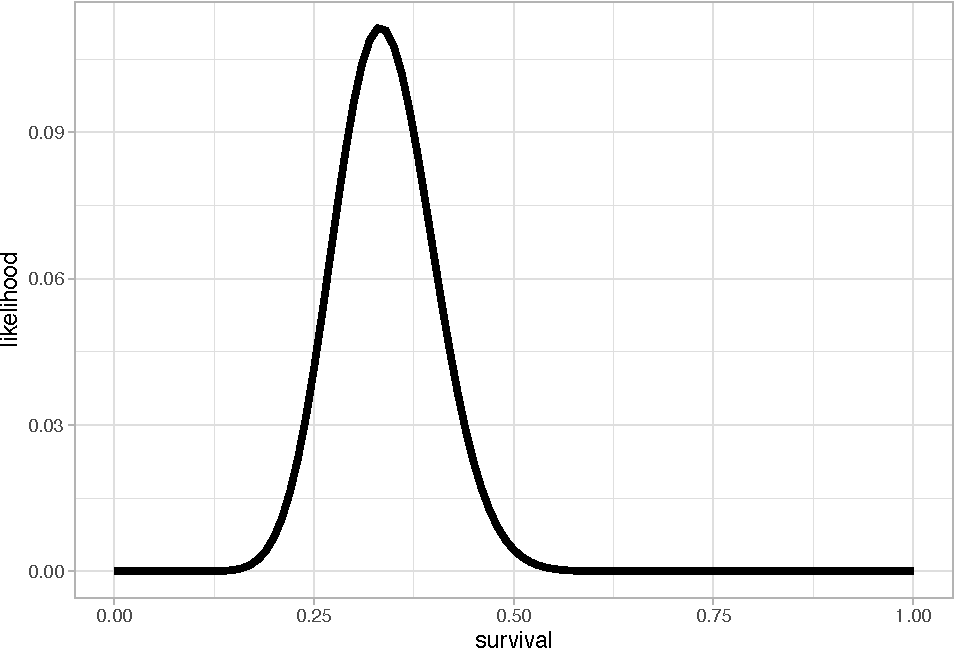
\includegraphics{banana-book_files/figure-latex/binlik-1.pdf}
\caption{\label{fig:binlik}Binomial likelihood with \(n = 57\) released animals and \(y = 19\) survivors after winter. The value of survival (on the x-axis) that corresponds to the maximum of the likelihood function (on the y-axis) is the MLE, or the proportion of success in this example, close to 0.33.}
\end{figure}

Besides the likelihood, priors are another component of the model in the Bayesian approach. For a parameter that is a probability, the one thing we know is that the prior should be a continuous random variable that lies between 0 and 1. To reflect that, we often go for the uniform distribution \(U(0,1)\) to imply \emph{vague} priors. Here vague means that survival has, before we see the data, the same probability of falling between 0.1 and 0.2 and between 0.8 and 0.9, for example.

\begin{align*}
\theta &\sim \text{Uniform}(0, 1) &\text{[prior for }\theta \text{]}
\end{align*}

Now we apply Bayes' theorem. We write a \texttt{R} function that computes the product of the likelihood times the prior, or the numerator in Bayes' theorem: \(\Pr(\text{data} \mid \theta) \times \Pr(\theta)\)

\begin{Shaded}
\begin{Highlighting}[]
\NormalTok{numerator }\OtherTok{\textless{}{-}} \ControlFlowTok{function}\NormalTok{(theta) }\FunctionTok{dbinom}\NormalTok{(y, n, theta) }\SpecialCharTok{*} \FunctionTok{dunif}\NormalTok{(theta, }\DecValTok{0}\NormalTok{, }\DecValTok{1}\NormalTok{)}
\end{Highlighting}
\end{Shaded}

We write another function that calculates the denominator, the average likelihood: \(\Pr(\text{data}) = \int{L(\theta \mid \text{data}) \Pr(\theta) d\theta}\)

\begin{Shaded}
\begin{Highlighting}[]
\NormalTok{denominator }\OtherTok{\textless{}{-}} \FunctionTok{integrate}\NormalTok{(numerator,}\DecValTok{0}\NormalTok{,}\DecValTok{1}\NormalTok{)}\SpecialCharTok{$}\NormalTok{value}
\end{Highlighting}
\end{Shaded}

We use the \texttt{R} function \texttt{integrate} to calculate the integral in the denominator, which implements quadrature techniques to divide in little squares the area underneath the curve delimited by the function to integrate (here the numerator), and count them.

Then we get a numerical approximation of the posterior in Figure \ref{fig:numapprox} by applying Bayes' theorem.

\begin{Shaded}
\begin{Highlighting}[]
\NormalTok{grid }\OtherTok{\textless{}{-}} \FunctionTok{seq}\NormalTok{(}\DecValTok{0}\NormalTok{, }\DecValTok{1}\NormalTok{, }\FloatTok{0.01}\NormalTok{) }\CommentTok{\# grid of values for theta}
\NormalTok{numerical\_posterior }\OtherTok{\textless{}{-}} \FunctionTok{data.frame}\NormalTok{(}\AttributeTok{survival =}\NormalTok{ grid, }
                                  \AttributeTok{posterior =} \FunctionTok{numerator}\NormalTok{(grid)}\SpecialCharTok{/}\NormalTok{denominator) }\CommentTok{\# Bayes\textquotesingle{} theorem}
\NormalTok{numerical\_posterior }\SpecialCharTok{\%\textgreater{}\%}
  \FunctionTok{ggplot}\NormalTok{() }\SpecialCharTok{+}
  \FunctionTok{aes}\NormalTok{(}\AttributeTok{x =}\NormalTok{ survival, }\AttributeTok{y =}\NormalTok{ posterior) }\SpecialCharTok{+} 
  \FunctionTok{geom\_line}\NormalTok{(}\AttributeTok{size =} \FloatTok{1.5}\NormalTok{)}
\end{Highlighting}
\end{Shaded}

\begin{figure}
\centering
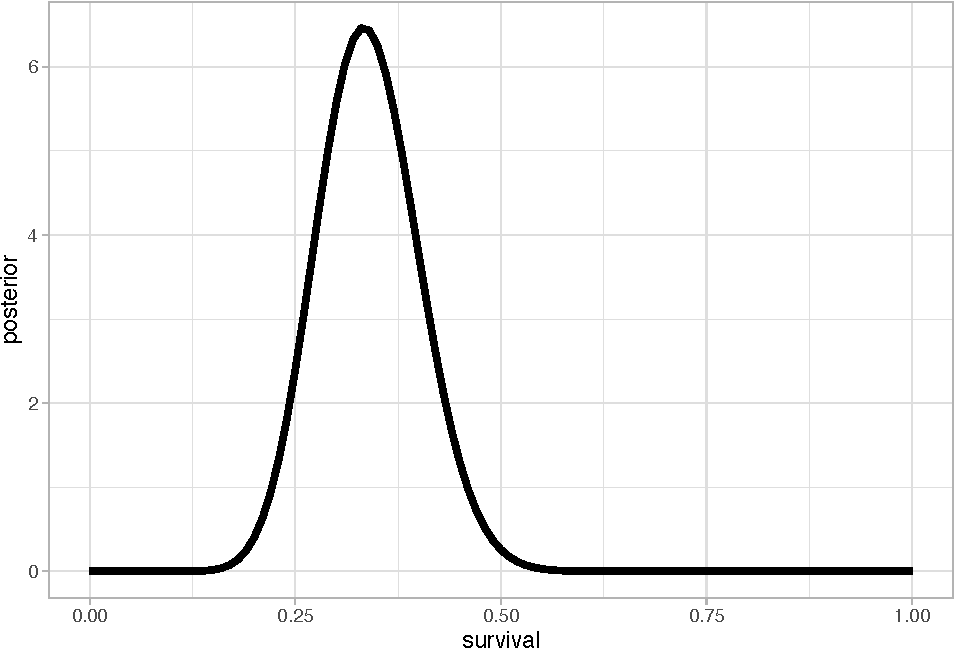
\includegraphics{banana-book_files/figure-latex/numapprox-1.pdf}
\caption{\label{fig:numapprox}Winter survival posterior distribution obtained by numerical integration.}
\end{figure}

How good is our numerical approximation of survival posterior distribution? Ideally, we would want to compare the approximation to the true posterior distribution. Although a closed-form expression for the posterior distribution is in general intractable, when you combine a binomial likelihood together with a beta distribution as a prior, then the posterior distribution is also a beta distribution, which makes it amenable to all sorts of exact calculations\footnote{We say that the beta distribution is the conjugate prior distribution for the binomial distribution.}. The beta distribution is continuous between 0 and 1, and extends the uniform distribution to situations where not all outcomes are equally likely. It has two parameters \(a\) and \(b\) that control its shape (Figure \ref{fig:betadistribution}).



\begin{figure}
\centering
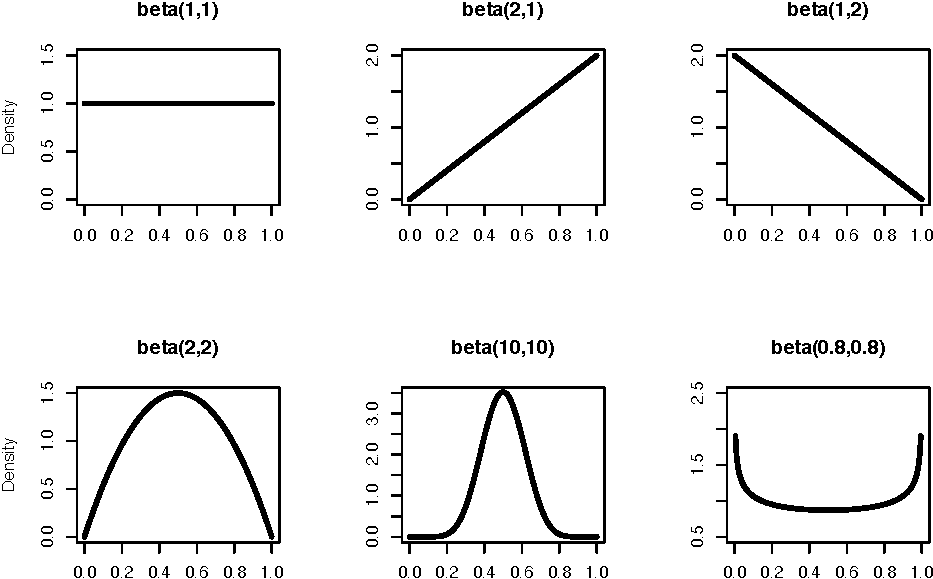
\includegraphics{banana-book_files/figure-latex/betadistribution-1.pdf}
\caption{\label{fig:betadistribution}The distribution beta(\(a\),\(b\)) for different values of \(a\) and \(b\). Note that for \(a = b = 1\), we get the uniform distribution between 0 and 1 in the top left panel. When \(a\) and \(b\) are equal, the distribution is symmetric, and the bigger \(a\) and \(b\), the more peaked the distribution or the smaller the variance.}
\end{figure}

If the likelihood of the data \(y\) is binomial with \(n\) trials and probability of success \(\theta\), and the prior is a beta distribution with parameters \(a\) and \(b\), then the posterior is a beta distribution with parameters \(a + y\) and \(b + n - y\)\footnote{\textbf{provide a sketch of the proof}}. In our example, we have \(n = 57\) trials and \(y = 19\) animals that survived and a uniform prior between 0 and 1 or a beta distribution with parameters \(a = b = 1\), therefore survival has a beta posterior distribution with parameters 20 and 39. In Figure \ref{fig:compar}, we superimpose the exact posterior and the numerical approximation. Clearly, the two distributions are indistinguishable, suggesting that the numerical approximation is more than fine.
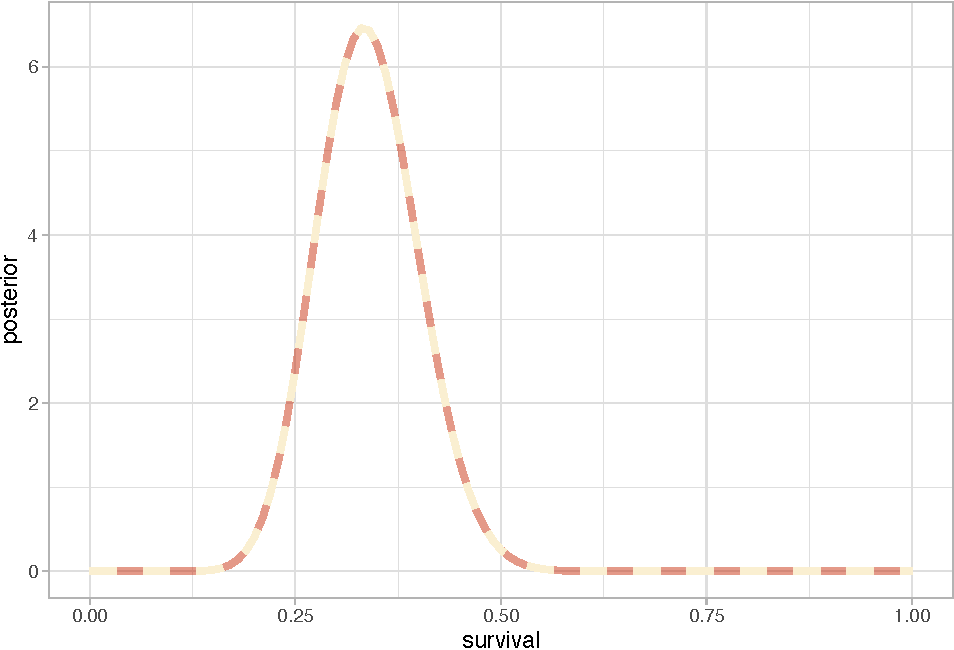
\includegraphics{banana-book_files/figure-latex/compar-1.pdf}

In our example, we have a single parameter to estimate, winter survival. This means dealing with a one-dimensional integral in the denominator which is pretty easy with quadrature techniques and the \texttt{R} function \texttt{integrate()}. Now what if we had multiple parameters? For example, imagine you'd like to fit a capture-recapture model with detection probability \(p\) and regression parameters \(\alpha\) and \(\beta\) for the intercept and slope of a relationship between survival probability and a covariate, then Bayes' theorem gives you the posterior distribution of all three parameters together:

\[ \Pr(\alpha, \beta, p \mid \text{data}) = \frac{ \Pr(\text{data} \mid \alpha, \beta, p) \times \Pr(\alpha, \beta, p)}{\iiint \, \Pr(\text{data} \mid \alpha, \beta, p) \Pr(\alpha, \beta, p) d\alpha d\beta dp} \]
There are two computational challenges with this formula. First, do we really wish to calculate a three-dimensional integral? The answer is no, one-dimensional and two-dimensional integrals are so much further we can go with standard methods. Second, we're more interested in a posterior distribution for each parameter separately than the joint posterior distribution. The so-called marginal distribution of \(p\) for example is obtained by integrating over all the other parameters -- a two-dimensional integral in this example. Now imagine with tens or hundreds of parameters to estimate, these integrals become highly multi-dimensional and simply intractable. In the next section, I introduce powerful simulation methods to circumvent this issue.

\hypertarget{markov-chain-monte-carlo-mcmc}{%
\section{Markov chain Monte Carlo (MCMC)}\label{markov-chain-monte-carlo-mcmc}}

In the early 1990s, statisticians rediscovered work from the 1950's in physics. In a famous paper that would lay the fundations of modern Bayesian statistics (Figure \ref{fig:mcmcpaper}), the authors use simulations to approximate posterior distributions with some precision by drawing large samples. This is a neat trick to avoid explicit calculation of the multi-dimensional integrals we struggle with when using Bayes' theorem.

\begin{figure}

{\centering 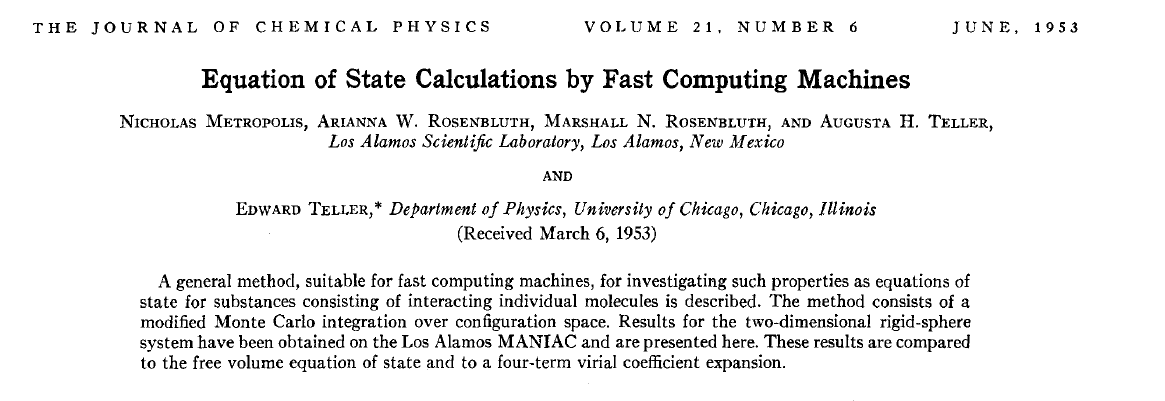
\includegraphics[width=16.18in]{images/metropolis} 

}

\caption{MCMC article cover. Source: [The Journal of Chemical Physics](https://aip.scitation.org/doi/10.1063/1.1699114)}\label{fig:mcmcpaper}
\end{figure}

These simulation algorithms are called Markov chain Monte Carlo (MCMC), and they definitely gave a boost to Bayesian statistics. There are two parts in MCMC, Markov chain and Monte Carlo, let's try and make sense of these terms.

\hypertarget{monte-carlo-integration}{%
\subsection{Monte Carlo integration}\label{monte-carlo-integration}}

What does Monte Carlo stand for? Monte Carlo integration is a simulation technique to calculate integrals of any function \(f\) of random variable \(X\) with distribution \(\Pr(X)\) say \(\int f(X) \Pr(X)dX\). You draw values \(X_1,\ldots,X_k\) from \(\Pr(X)\) the distribution of \(X\), apply function \(f\) to these values, then calculate the mean of these new values \(\displaystyle{\frac{1}{k}}\sum_{i=1}^k{f(X_i)}\) to approximate the integral. How is Monte Carlo integration used in a Bayesian context? The posterior distribution contains all the information we need about the parameter to be estimated. When dealing with many parameters however, you may want to summarise posterior results by calculating numerical summaries. The simplest numerical summary is the mean of the posterior distribution, \(E(\theta) = \int \theta \Pr(\theta|\text{data})\), where \(X\) is \(\theta\) now and \(f\) is the identity function. Posterior mean can be calculated with Monte Carlo integration:

\begin{Shaded}
\begin{Highlighting}[]
\NormalTok{sample\_from\_posterior }\OtherTok{\textless{}{-}} \FunctionTok{rbeta}\NormalTok{(}\DecValTok{1000}\NormalTok{, }\DecValTok{20}\NormalTok{, }\DecValTok{39}\NormalTok{) }\CommentTok{\# draw 1000 values from posterior survival beta(20,39)}
\FunctionTok{mean}\NormalTok{(sample\_from\_posterior) }\CommentTok{\# compute mean with Monte Carlo integration}
\DocumentationTok{\#\# [1] 0.3396}
\end{Highlighting}
\end{Shaded}

You may check that the mean we have just calculated matches closely the expectation of a beta distribution\footnote{If \(X\) is a random variable with distribution \(\text{beta}(a, b)\), then \(E(X) = \displaystyle{\frac{a}{a + b}}\)}:

\begin{Shaded}
\begin{Highlighting}[]
\DecValTok{20}\SpecialCharTok{/}\NormalTok{(}\DecValTok{20}\SpecialCharTok{+}\DecValTok{39}\NormalTok{) }\CommentTok{\# expectation of beta(20,39)}
\DocumentationTok{\#\# [1] 0.339}
\end{Highlighting}
\end{Shaded}

Another useful numerical summary is the credible interval within which our parameter falls with some probability, usually 0.95 hence a 95\(\%\) credible interval. Finding the bounds of a credible interval requires calculating quantiles, which in turn involves integrals and the use of Monte Carlo integration. A 95\(\%\) credible interval for winter survival can be obtained in \texttt{R} with:

\begin{Shaded}
\begin{Highlighting}[]
\FunctionTok{quantile}\NormalTok{(sample\_from\_posterior, }\AttributeTok{probs =} \FunctionTok{c}\NormalTok{(}\FloatTok{2.5}\SpecialCharTok{/}\DecValTok{100}\NormalTok{, }\FloatTok{97.5}\SpecialCharTok{/}\DecValTok{100}\NormalTok{))}
\DocumentationTok{\#\#   2.5\%  97.5\% }
\DocumentationTok{\#\# 0.2264 0.4572}
\end{Highlighting}
\end{Shaded}

\hypertarget{markov-chains}{%
\subsection{Markov chains}\label{markov-chains}}

What is a Markov chain? A Markov chain is a random sequence of numbers, in which each number depends only on the previous number. An example is the weather in my home town in Southern France, Montpellier, in which a sunny day is most likely to be followed by another sunny day, say with probability 0.8, and a rainy day is rarely followed by another rainy day, say with probability 0.1. The dynamic of this Markov chain is captured by the transition matrix \(\mathbf{\Gamma}\):
\[
\begin{matrix}
& \\
\mathbf{\Gamma} = 
    \left ( \vphantom{ \begin{matrix} 12 \\ 12 \end{matrix} } \right .
\end{matrix}
\hspace{-1.2em}
\begin{matrix}
    \text{sunny tomorrow} & \text{rainy tomorrow} \\ 
0.8 & 0.2 \\ 
0.9 & 0.1 \\ 
\end{matrix}
\hspace{-0.2em}
\begin{matrix}
& \\
\left . \vphantom{ \begin{matrix} 12 \\ 12 \\ 12 \end{matrix} } \right )
    \begin{matrix}
    \text{sunny today} \\ \text{rainy today}
    \end{matrix}
\end{matrix}
\]
In rows the weather today, and in columns the weather tomorrow. The cells give the probability of a sunny or rainy day tomorrow, given the day is sunny or rainy today. Under certain conditions\footnote{The Markov chain is irreducible and aperiodic.}, a Markov chain will converge to a unique stationary distribution. In our weather example, let's run the Markov chain for 20 steps:

\begin{Shaded}
\begin{Highlighting}[]
\NormalTok{weather }\OtherTok{\textless{}{-}} \FunctionTok{matrix}\NormalTok{(}\FunctionTok{c}\NormalTok{(}\FloatTok{0.8}\NormalTok{, }\FloatTok{0.2}\NormalTok{, }\FloatTok{0.9}\NormalTok{, }\FloatTok{0.1}\NormalTok{), }\AttributeTok{nrow =} \DecValTok{2}\NormalTok{, }\AttributeTok{byrow =}\NormalTok{ T) }\CommentTok{\# transition matrix}
\NormalTok{steps }\OtherTok{\textless{}{-}} \DecValTok{20}
\ControlFlowTok{for}\NormalTok{ (i }\ControlFlowTok{in} \DecValTok{1}\SpecialCharTok{:}\NormalTok{steps)\{}
\NormalTok{  weather }\OtherTok{\textless{}{-}}\NormalTok{ weather }\SpecialCharTok{\%*\%}\NormalTok{ weather }\CommentTok{\# matrix multiplication}
\NormalTok{\}}
\FunctionTok{round}\NormalTok{(weather, }\DecValTok{2}\NormalTok{) }\CommentTok{\# matrix product after 20 steps}
\DocumentationTok{\#\#      [,1] [,2]}
\DocumentationTok{\#\# [1,] 0.82 0.18}
\DocumentationTok{\#\# [2,] 0.82 0.18}
\end{Highlighting}
\end{Shaded}

Each row of the transition matrix converges to the same distribution \((0.82, 0.18)\) as the number of steps increases. Convergence happens no matter which state you start in, and you always have probability 0.82 of the day being sunny and 0.18 of the day being rainy.

Back to MCMC, the core idea is that you can build a Markov chain with a given stationary distribution set to be the desired posterior distribution.

\begin{rmdnote}
Putting Monte Carlo and Markov chains together, MCMC allows us to generate a sample of values (Markov chain) whose distribution converges to the posterior distribution, and we can use this sample of values to calculate any posterior summaries (Monte Carlo), such as posterior means and credible intervals.
\end{rmdnote}

\hypertarget{metropolis-algorithm}{%
\subsection{Metropolis algorithm}\label{metropolis-algorithm}}

There are several ways of constructing Markov chains for Bayesian inference\footnote{You might have heard about the Metropolis-Hastings or the Gibbs sampler. Have a look to \url{https://github.com/chi-feng/mcmc-demo} for an interactive gallery of MCMC algorithms.}. Here I illustrate the Metropolis algorithm and how to implement it in practice\footnote{This presentation is largely inspired by \citet{alberthu2019}}.

Let's go back to our example on animal survival estimation. We illustrate sampling from survival posterior distribution. We write functions for likelihood, prior and posterior.

\begin{Shaded}
\begin{Highlighting}[]
\CommentTok{\# 19 animals recaptured alive out of 57 captured, marked and released}
\NormalTok{survived }\OtherTok{\textless{}{-}} \DecValTok{19}
\NormalTok{released }\OtherTok{\textless{}{-}} \DecValTok{57}

\CommentTok{\# binomial log{-}likelihood function}
\NormalTok{loglikelihood }\OtherTok{\textless{}{-}} \ControlFlowTok{function}\NormalTok{(x, p)\{}
  \FunctionTok{dbinom}\NormalTok{(}\AttributeTok{x =}\NormalTok{ x, }\AttributeTok{size =}\NormalTok{ released, }\AttributeTok{prob =}\NormalTok{ p, }\AttributeTok{log =} \ConstantTok{TRUE}\NormalTok{)}
\NormalTok{\}}

\CommentTok{\# uniform prior density}
\NormalTok{logprior }\OtherTok{\textless{}{-}} \ControlFlowTok{function}\NormalTok{(p)\{}
  \FunctionTok{dunif}\NormalTok{(}\AttributeTok{x =}\NormalTok{ p, }\AttributeTok{min =} \DecValTok{0}\NormalTok{, }\AttributeTok{max =} \DecValTok{1}\NormalTok{, }\AttributeTok{log =} \ConstantTok{TRUE}\NormalTok{)}
\NormalTok{\}}

\CommentTok{\# posterior density function (log scale)}
\NormalTok{posterior }\OtherTok{\textless{}{-}} \ControlFlowTok{function}\NormalTok{(x, p)\{}
  \FunctionTok{loglikelihood}\NormalTok{(x, p) }\SpecialCharTok{+} \FunctionTok{logprior}\NormalTok{(p) }\CommentTok{\# {-} log(Pr(data))}
\NormalTok{\}}
\end{Highlighting}
\end{Shaded}

The Metropolis algorithm works as follows:

\begin{enumerate}
\def\labelenumi{\arabic{enumi}.}
\item
  We pick a value of the parameter to be estimated. This is where we start our Markov chain -- this is a \emph{starting} value.
\item
  To decide where to go next, we propose to move away from the current value of the parameter -- this is a \emph{candidate} value. To do so, we add to the current value some random value from e.g.~a normal distribution with some variance -- this is a \emph{proposal} distribution. The Metropolis algorithm is a particular case of the Metropolis-Hastings algorithm with symmetric proposals.
\item
  We compute the ratio of the probabilities at the candidate and current locations \(R=\displaystyle{\frac{{\Pr(\text{candidate}|\text{data})}}{{\Pr(\text{current}|\text{data})}}}\). This is where the magic of MCMC happens, in that \(\Pr(\text{data})\), the denominator in the Bayes' theorem, appears in both the numerator and the denominator in \(R\) therefore cancels out and does not need to be calculated.
\end{enumerate}

\begin{enumerate}
\def\labelenumi{\arabic{enumi}.}
\setcounter{enumi}{3}
\item
  If the posterior at the candidate location \(\Pr(\text{candidate}|\text{data})\) is higher than at the current location \(\Pr(\text{current}|\text{data})\), in other words when the candidate value is more plausible than the current value, we definitely accept the candidate value. If not, then we accept the candidate value with probability \(R\) and reject with probability \(1-R\). For example, if the candidate value is ten times less plausible than the current value, then we accept with probability 0.1 and reject with probability 0.9. How does it work in practice? We use a continuous spinner that lands somewhere between 0 and 1 -- call the random spin \(X\). If \(X\) is smaller than \(R\), we move to the candidate location, otherwise we remain at the current location. We do not want to accept or reject too often. In practice, the Metropolis algorithm should have an acceptance probability between 0.2 and 0.4, which can be achieved by \emph{tuning} the variance of the normal proposal distribution.
\item
  We repeat 2-4 a number of times -- or \emph{steps}.
\end{enumerate}

Enough of the theory, let's implement the Metropolis algorithm in \texttt{R}. Let's start by setting the scene.

\begin{Shaded}
\begin{Highlighting}[]
\NormalTok{steps }\OtherTok{\textless{}{-}} \DecValTok{100} \CommentTok{\# number of steps}
\NormalTok{theta.post }\OtherTok{\textless{}{-}} \FunctionTok{rep}\NormalTok{(}\ConstantTok{NA}\NormalTok{, steps) }\CommentTok{\# vector to store samples}
\NormalTok{accept }\OtherTok{\textless{}{-}} \FunctionTok{rep}\NormalTok{(}\ConstantTok{NA}\NormalTok{, steps) }\CommentTok{\# keep track of accept/reject}
\FunctionTok{set.seed}\NormalTok{(}\DecValTok{1234}\NormalTok{) }\CommentTok{\# for reproducibility}
\end{Highlighting}
\end{Shaded}

Now follow the 5 steps we've just described. First, we pick a starting value, and store it (step 1).

\begin{Shaded}
\begin{Highlighting}[]
\NormalTok{inits }\OtherTok{\textless{}{-}} \FloatTok{0.5}
\NormalTok{theta.post[}\DecValTok{1}\NormalTok{] }\OtherTok{\textless{}{-}}\NormalTok{ inits}
\NormalTok{accept[}\DecValTok{1}\NormalTok{] }\OtherTok{\textless{}{-}} \DecValTok{1}
\end{Highlighting}
\end{Shaded}

Then, we need a function to propose a candidate value. We add a value taken from a normal distribution with mean zero and standard deviation we call \emph{away}. We work on the logit scale to make sure the candidate value for survival lies between 0 and 1.

\begin{Shaded}
\begin{Highlighting}[]
\NormalTok{move }\OtherTok{\textless{}{-}} \ControlFlowTok{function}\NormalTok{(x, }\AttributeTok{away =} \DecValTok{1}\NormalTok{)\{ }\CommentTok{\# by default, standard deviation of the proposal distribution is 1}
\NormalTok{  logitx }\OtherTok{\textless{}{-}} \FunctionTok{log}\NormalTok{(x }\SpecialCharTok{/}\NormalTok{ (}\DecValTok{1} \SpecialCharTok{{-}}\NormalTok{ x)) }\CommentTok{\# apply logit transform ({-}infinity,+infinity)}
\NormalTok{  logit\_candidate }\OtherTok{\textless{}{-}}\NormalTok{ logitx }\SpecialCharTok{+} \FunctionTok{rnorm}\NormalTok{(}\DecValTok{1}\NormalTok{, }\DecValTok{0}\NormalTok{, away) }\CommentTok{\# add a value taken from N(0,sd=away) to current value}
\NormalTok{  candidate }\OtherTok{\textless{}{-}} \FunctionTok{plogis}\NormalTok{(logit\_candidate) }\CommentTok{\# back{-}transform (0,1)}
  \FunctionTok{return}\NormalTok{(candidate)}
\NormalTok{\}}
\end{Highlighting}
\end{Shaded}

Now we're ready for steps 2, 3 and 4. We write a loop to take care of step 5. We start at initial value 0.5 and run the algorithm for 100 steps or iterations.

\begin{Shaded}
\begin{Highlighting}[]
\ControlFlowTok{for}\NormalTok{ (t }\ControlFlowTok{in} \DecValTok{2}\SpecialCharTok{:}\NormalTok{steps)\{ }\CommentTok{\# repeat steps 2{-}4 (step 5)}
  
  \CommentTok{\# propose candidate value for survival (step 2)}
\NormalTok{  theta\_star }\OtherTok{\textless{}{-}} \FunctionTok{move}\NormalTok{(theta.post[t}\DecValTok{{-}1}\NormalTok{])}
  
  \CommentTok{\# calculate ratio R (step 3)}
\NormalTok{  pstar }\OtherTok{\textless{}{-}} \FunctionTok{posterior}\NormalTok{(survived, }\AttributeTok{p =}\NormalTok{ theta\_star)  }
\NormalTok{  pprev }\OtherTok{\textless{}{-}} \FunctionTok{posterior}\NormalTok{(survived, }\AttributeTok{p =}\NormalTok{ theta.post[t}\DecValTok{{-}1}\NormalTok{])}
\NormalTok{  logR }\OtherTok{\textless{}{-}}\NormalTok{ pstar }\SpecialCharTok{{-}}\NormalTok{ pprev }\CommentTok{\# likelihood and prior are on the log scale}
\NormalTok{  R }\OtherTok{\textless{}{-}} \FunctionTok{exp}\NormalTok{(logR)}
  
  \CommentTok{\# accept candidate value or keep current value (step 4)}
\NormalTok{  X }\OtherTok{\textless{}{-}} \FunctionTok{runif}\NormalTok{(}\DecValTok{1}\NormalTok{, }\DecValTok{0}\NormalTok{, }\DecValTok{1}\NormalTok{) }\CommentTok{\# spin continuous spinner}
  \ControlFlowTok{if}\NormalTok{ (X }\SpecialCharTok{\textless{}}\NormalTok{ R)\{}
\NormalTok{    theta.post[t] }\OtherTok{\textless{}{-}}\NormalTok{ theta\_star }\CommentTok{\# accept candidate value}
\NormalTok{    accept[t] }\OtherTok{\textless{}{-}} \DecValTok{1} \CommentTok{\# accept}
\NormalTok{  \}}
  \ControlFlowTok{else}\NormalTok{\{}
\NormalTok{    theta.post[t] }\OtherTok{\textless{}{-}}\NormalTok{ theta.post[t}\DecValTok{{-}1}\NormalTok{] }\CommentTok{\# keep current value}
\NormalTok{    accept[t] }\OtherTok{\textless{}{-}} \DecValTok{0} \CommentTok{\# reject}
\NormalTok{  \}}
\NormalTok{\}}
\end{Highlighting}
\end{Shaded}

We get the following values.

\begin{Shaded}
\begin{Highlighting}[]
\FunctionTok{head}\NormalTok{(theta.post) }\CommentTok{\# first values}
\DocumentationTok{\#\# [1] 0.5000 0.2302 0.2906 0.2906 0.2980 0.2980}
\FunctionTok{tail}\NormalTok{(theta.post) }\CommentTok{\# last values}
\DocumentationTok{\#\# [1] 0.2622 0.2622 0.2622 0.3727 0.3232 0.3862}
\end{Highlighting}
\end{Shaded}

Visually, you may look at the chain in Figure \ref{fig:chain} called a trace plot.

\begin{figure}

{\centering 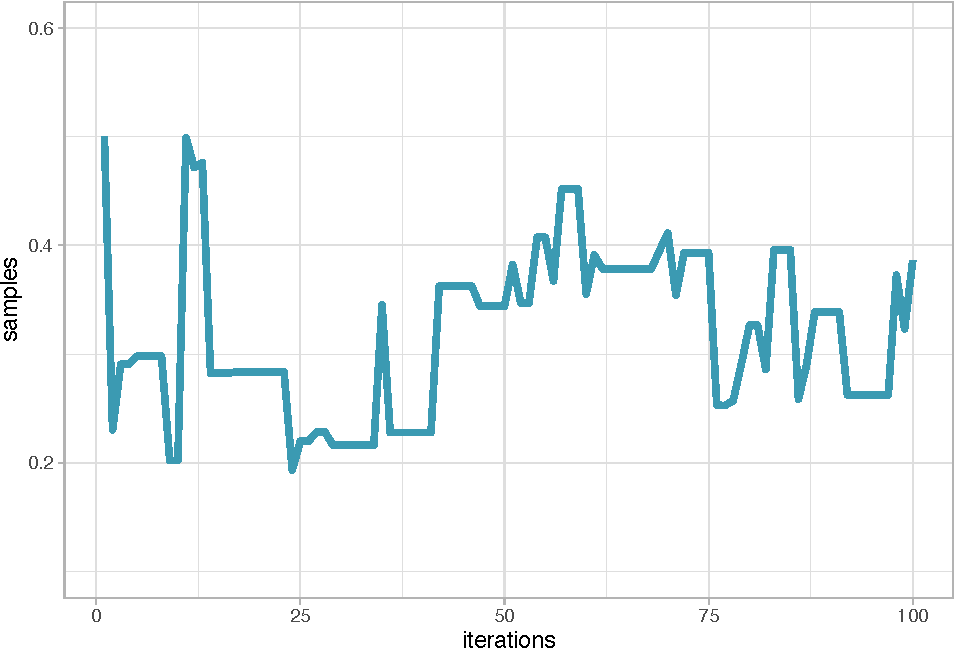
\includegraphics{banana-book_files/figure-latex/chain-1} 

}

\caption{Visualisation of a Markov chain starting at value 0.5, with steps or iterations on the x-axis, and samples on the y-axis. This graphical representation is called a trace plot.}\label{fig:chain}
\end{figure}

The acceptance probability is the average number of times we accepted a candidated value, which is 0.44 and almost satisfying.

Can we run another chain and start at initial value 0.2 this time? Yes, just go through the same algorithm again, and visualise the results in Figure \ref{fig:twochains}.

\begin{figure}

{\centering 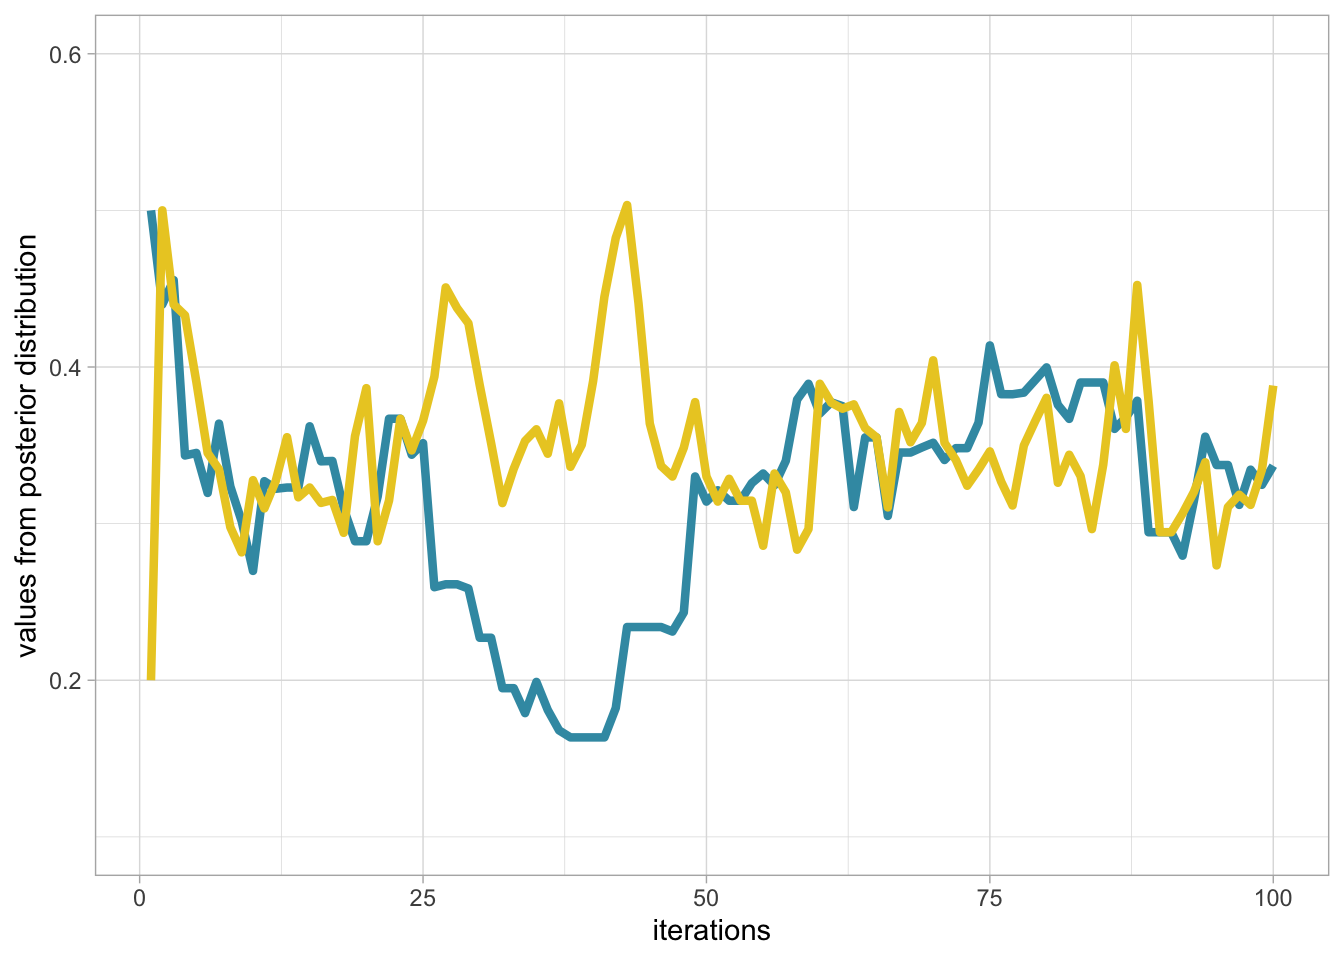
\includegraphics{banana-book_files/figure-latex/twochains-1} 

}

\caption{Trace plot of survival for two chains starting at 0.2 (yellow) and 0.5 (blue) run for 100 steps.}\label{fig:twochains}
\end{figure}

Notice that we do not get the exact same results because the algorithm is stochastic. The question is to know whether we have reached the stationary distribution. Let's increase the number of steps and run a chain with 5000 iterations as in Figure \ref{fig:longchain}.

\begin{figure}

{\centering 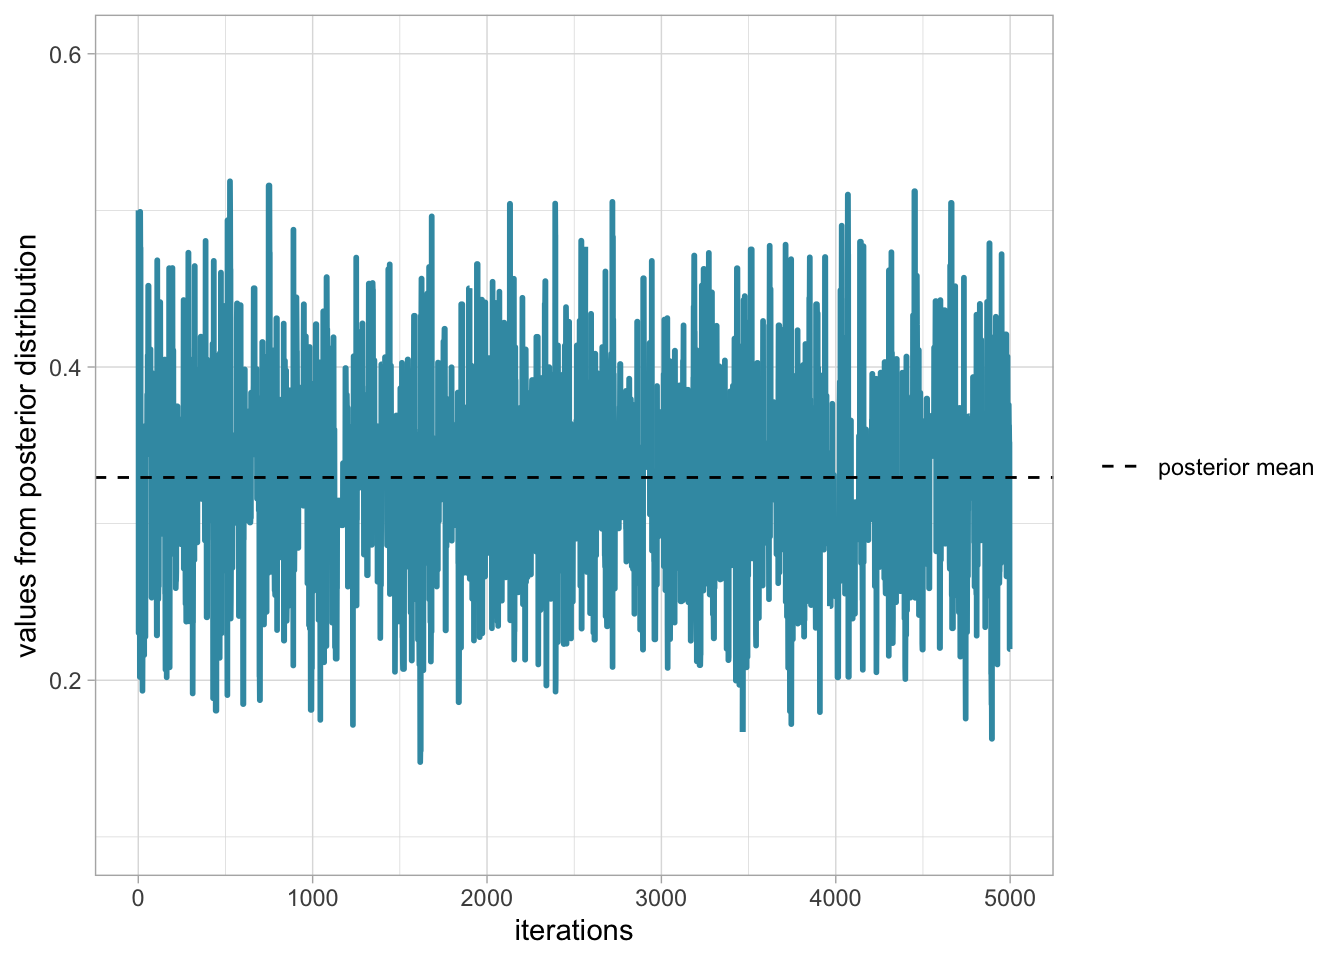
\includegraphics{banana-book_files/figure-latex/longchain-1} 

}

\caption{Trace plot of survival for a chain starting at 0.5 and 1000 steps.}\label{fig:longchain}
\end{figure}

This is what we're after, a trace plot that looks like a beautiful lawn, see Section \ref{convergence-diag}. I find it informative to look at the animated version of Figure \ref{fig:longchain}, it helps understanding the stochastic behavior of the algorithm, and also to realise how the chains converge to their stationary distribution, see Figure \ref{fig:animlongchain}.

\begin{figure}

{\centering \includegraphics[width=1\linewidth]{images/traceplotMCMC} 

}

\caption{Animated trace plot of survival with three chains starting at 0.2, 0.5 and 0.7 run for 1000 steps.}\label{fig:animlongchain}
\end{figure}

Once the stationary distribution is reached, you may regard the realisations of the Markov chain as a sample from the posterior distribution, and obtain numerical summaries. In the next section, we consider several important implementation issues.

\hypertarget{convergence-diag}{%
\section{Assessing convergence}\label{convergence-diag}}

\begin{rmdnote}
When implementing MCMC, we need to determine how long it takes for our Markov chain to converge to the target distribution, and the number of iterations we need after achieving convergence to get reasonable Monte Carlo estimates of numerical summaries (posterior means and credible intervals).
\end{rmdnote}

\hypertarget{burn-in}{%
\subsection{Burn-in}\label{burn-in}}

In practice, we discard observations from the start of the Markov chain and just use observations from the chain once it has converged. The initial observations that we discard are usually referred to as the \emph{burn-in}.

The simplest method to determine the length of the burn-in period is to look at trace plots. Going back to our example, we see from the trace plot in Figure \ref{fig:burnin} that we need at least 100 iterations to achieve convergence toward an average survival around 0.3. It is always better to be conservative when specifying the length of the burn-in period, and in this example, we would use 250 or even 500 iterations as a burn-in. The length of the burn-in period can be determined by performing preliminary MCMC short runs.

\begin{figure}
\centering
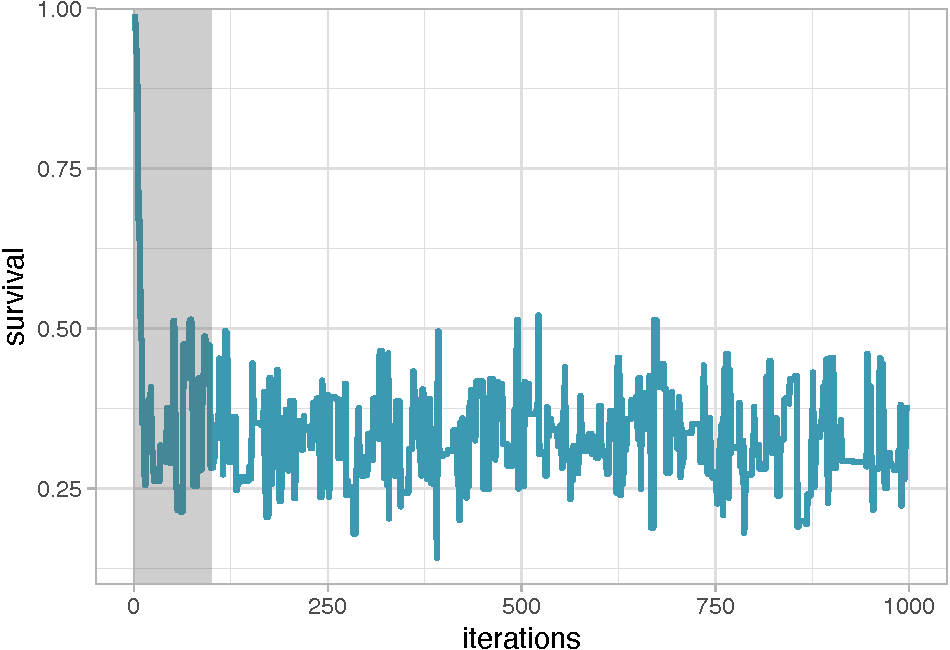
\includegraphics{banana-book_files/figure-latex/burnin-1.pdf}
\caption{\label{fig:burnin}Determining the length of the burn-in period. The chain starts at value 0.99 and rapidly stabilises, with values bouncing back and forth around 0.3 from the 100th iteration onwards. You may choose the shaded area as the burn-in, and discard the corresponding values.}
\end{figure}

Inspecting the trace plot for a single run of the Markov chain is useful. However, we usually run the Markov chain several times, starting from different over-dispersed points, to check that all runs achieve the same stationary distribution. This approach is formalised by using the Brooks-Gelman-Rubin (BGR) statistic \(\hat{R}\) which measures the ratio of the total variability combining multiple chains (between-chain plus within-chain) to the within-chain variability. The BGR statistic asks whether there is a chain effect, and is very much alike the \(F\) test in an analysis of variance. Values below 1.1 indicate likely convergence.

Back to our example, we run two Markov chains with starting values 0.2 and 0.8 using 100 up to 5000 iterations, and calculate the BGR statistic using half the number of iterations as the length of the burn-in. From Figure \ref{fig:bgr}, we get a value of the BGR statistic near 1 by up to 2000 iterations, which suggests that with 2000 iterations as a burn-in, there is no evidence of a lack of convergence.

\begin{figure}
\centering
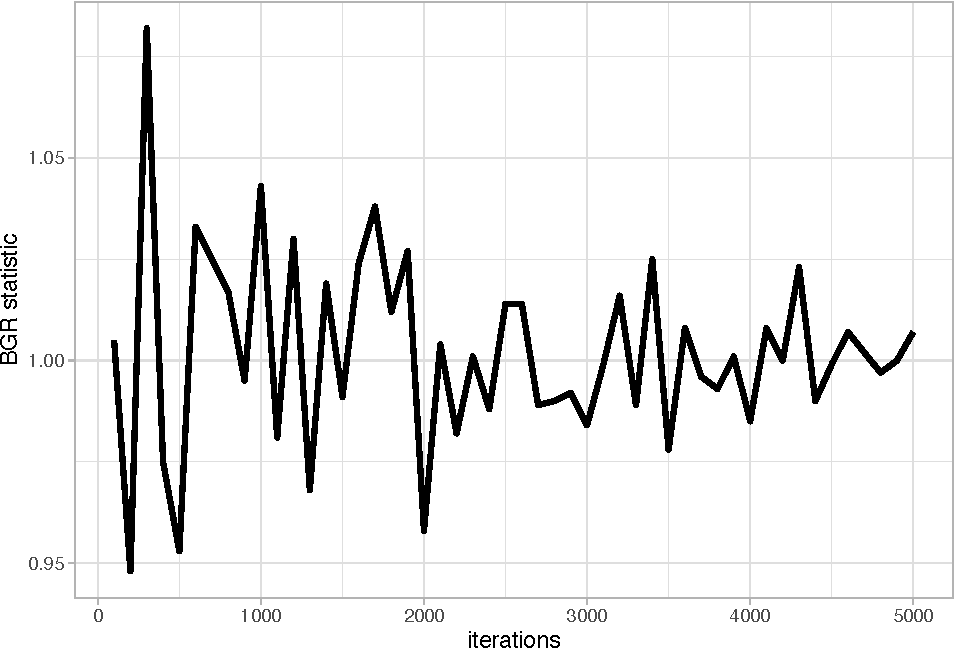
\includegraphics{banana-book_files/figure-latex/bgr-1.pdf}
\caption{\label{fig:bgr}Brooks-Gelman-Rubin statistic as a function of the number of iterations.}
\end{figure}

It is important to bear in mind that a value near 1 for the BGR statistic is only a necessary \emph{but not sufficient} condition for convergence. In other words, this diagnostic cannot tell you for sure that the Markov chain has achieved convergence, only that it has not.\footnote{Cross-reference sections on local minima and parameter redundancy for pathological cases.}

\hypertarget{chain-length}{%
\subsection{Chain length}\label{chain-length}}

How long of a chain is needed to produce reliable parameter estimates? To answer this question, you need to keep in mind that successive steps in a Markov chain are not independent -- this is usually referred to as \emph{autocorrelation}. Ideally, we would like to keep autocorrelation as low as possible. Here again, trace plots are useful to diagnose issues with autocorrelation. Let's get back to our survival example. Figure \ref{fig:tracechainlength} shows trace plots for different values of the standard deviation (parameter \emph{away}) of the (normal) proposal distribution we use to propose a candidate value (Section \ref{metropolis-algorithm}). Small and big moves provide high correlations between successive observations of the Markov chain, whereas a standard deviation of 1 allows efficient exploration of the parameter space. The movement around the parameter space is referred to as \emph{mixing}. Mixing is bad when the chain makes small and big moves, and good otherwise.

\begin{figure}
\centering
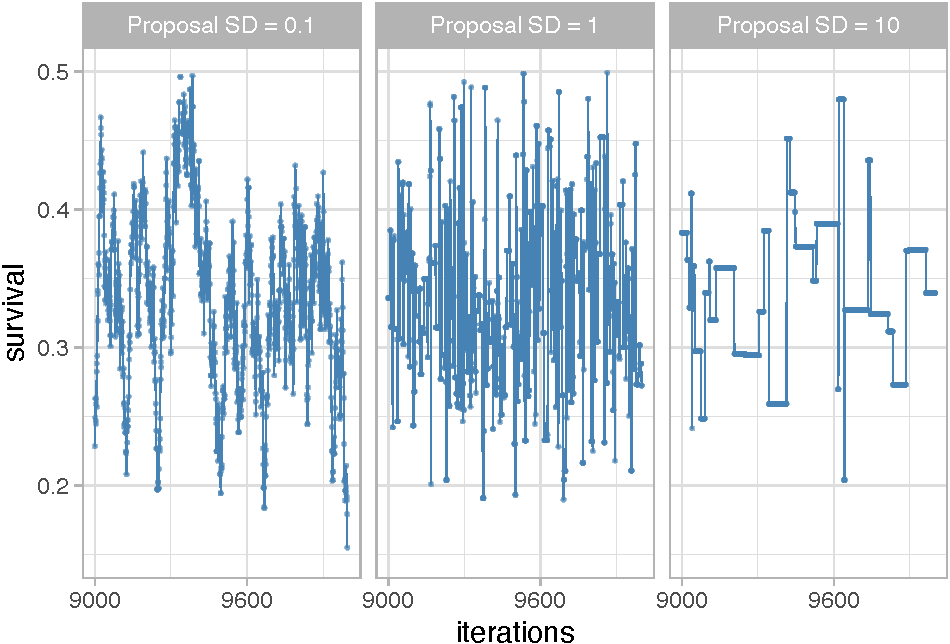
\includegraphics{banana-book_files/figure-latex/tracechainlength-1.pdf}
\caption{\label{fig:tracechainlength}Trace plots for different values of the standard deviation (SD) of the proposal distribution. Left: The chain exhibits small moves and mixing is bad. Right: The chain exhibits big moves and mixing is bad. Middle: The chain exhibits adequate moves and mixing is good. Only the thousand last iterations are shown.}
\end{figure}

In addition to trace plots, autocorrelation function (ACF) plots are a convenient way of displaying the strength of autocorrelation in a given sample values. ACF plots provide the autocorrelation between successively sampled values separated by an increasing number of iterations, or \emph{lag} (Figure \ref{fig:acfchainlength}).

\begin{figure}
\centering
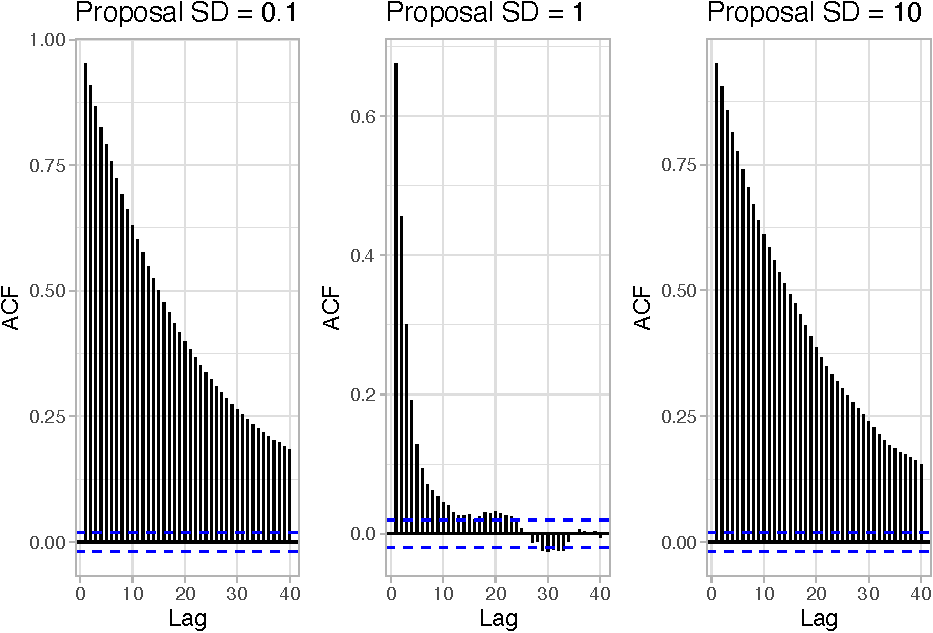
\includegraphics{banana-book_files/figure-latex/acfchainlength-1.pdf}
\caption{\label{fig:acfchainlength}Autocorrelation function plots for different values of the standard deviation (SD) of the proposal distribution. Left and right: Autocorrelation is strong, decreases slowly with increasing lag and mixing is bad. Middle: Autocorrelation is weak, decreases rapidly with increasing lag and mixing is good.}
\end{figure}

Autocorrelation is not necessarily a big issue. Strongly correlated observations just require large sample sizes and therefore longer simulations. But how many iterations exactly? The effective sample size (\texttt{n.eff}) measures chain length while taking into account chain autocorrelation. You should check the \texttt{n.eff} of every parameter of interest, and of any interesting parameter combinations. In general, we need \(\text{n.eff} \geq 1000\) independent steps to get reasonable Monte Carlo estimates of model parameters. In the animal survival example, \texttt{n.eff} can be calculated with the R \texttt{coda::effectiveSize()} function.

\begin{longtable}[]{@{}rr@{}}
\toprule
Proposal SD & n.eff \\
\midrule
\endhead
0.1 & 224 \\
1.0 & 1934 \\
10.0 & 230 \\
\bottomrule
\end{longtable}

As expected, \texttt{n.eff} is less than the number of MCMC iterations because of autocorrelation. Only when the standard deviation of the proposal distribution is 1 and mixing is good (Figures \ref{fig:tracechainlength} and \ref{fig:acfchainlength}) we get a satisfying effective sample size.

\hypertarget{what-if-you-have-issues-of-convergence}{%
\subsection{What if you have issues of convergence?}\label{what-if-you-have-issues-of-convergence}}

When diagnosing MCMC convergence, you will (very) often run into troubles. In this section you will find some helpful tips I hope.

When mixing is bad and effective sample size is small, you may just need to increase burn-in and/or sample more. Using more informative priors might also make Markov chains converge faster by helping your MCMC sampler (e.g.~the Metropolis algorithm) navigating more efficiently the parameter space. In the same spirit, picking better initial values for starting the chain does not harm. For doing that, a strategy consists in using estimates from a simpler model for which your MCMC chains do converge.

If convergence issues persist, often there is a problem with your model\footnote{The quote `When you have computational problems, often there's a problem with your model' is the folk theorem of statistical computing stated by Andrew Gelman in 2008, see \url{https://statmodeling.stat.columbia.edu/2008/05/13/the_folk_theore/}}. A bug in the code? A typo somewhere? A mistake in your maths? As often when coding is involved, the issue can be identified by removing complexities, and start with a simpler model until you find what the problem is.

A general advice is to see your model as a data generating tool in the first place, simulate data from it using some realistic values for the parameters, and try to recover these parameter values by fitting the model to the simulated data. Simulating from a model will help you understanding how it works, what it does not do, and the data you need to get reasonable parameter estimates.

We will see other strategies to improve convergence in the next chapters.\footnote{Cross reference relevant chapters. Option 1. Change your sampler. Option 2. Reparameterize (standardize covariates, plus non-centering: \(\alpha \sim N(0,\sigma)\) becomes \(\alpha = z \sigma\) with \(z \sim N(0,1)\)).}

\hypertarget{summary}{%
\section{Summary}\label{summary}}

\begin{itemize}
\item
  With the Bayes' theorem, you update your beliefs (prior) with new data (likelihood) to get posterior beliefs (posterior): posterior \(\propto\) likelihood \(\times\) prior.
\item
  The idea of Markov chain Monte Carlo (MCMC) is to simulate values from a Markov chain which has a stationary distribution equal to the posterior distribution you're after.
\item
  In practice, you run a Markov chain multiple times starting from over-dispersed initial values.
\item
  You discard iterations in an initial burn-in phase and achieve convergence when all chains reach the same regime.
\item
  From there, you run the chains long enough and proceed with calculating Monte Carlo estimates of numerical summaries (e.g.~posterior means and credible intervals) for parameters.
\end{itemize}

\hypertarget{suggested-reading}{%
\section{Suggested reading}\label{suggested-reading}}

\begin{itemize}
\item
  Gelman, A. and Hill, J. (2006). \href{https://www.cambridge.org/core/books/data-analysis-using-regression-and-multilevelhierarchical-models/32A29531C7FD730C3A68951A17C9D983}{Data Analysis Using Regression and Multilevel/Hierarchical Models (Analytical Methods for Social Research)}. Cambridge: Cambridge University Press.
\item
  Gelman, A. and colleagues (2020). \href{https://arxiv.org/pdf/2011.01808.pdf}{Bayesian workflow}. arXiv preprint.
\item
  McCarthy, M. (2007). \href{https://www.cambridge.org/core/books/bayesian-methods-for-ecology/9225F65B8A25D69B0B6C50B5A9A78201}{Bayesian Methods for Ecology}. Cambridge: Cambridge University Press.
\item
  McElreath, R. (2020). \href{https://xcelab.net/rm/statistical-rethinking/}{Statistical Rethinking: A Bayesian Course with Examples in R and Stan (2nd ed.)}. CRC Press.
\end{itemize}

\hypertarget{intronimble}{%
\chapter{NIMBLE tutorial}\label{intronimble}}

\hypertarget{introduction-2}{%
\section{Introduction}\label{introduction-2}}

In this second chapter, you will get familiar with NIMBLE an R package that implements up-to-date MCMC algorithms for fitting complex models. NIMBLE spares you from coding the MCMC algorithms by hand, and only requires the specification of a likelihood and priors for model parameters. You will go through a simple example to illustrate NIMBLE main features, but the ideas hold for other problems.

\hypertarget{what-is-nimble}{%
\section{What is NIMBLE?}\label{what-is-nimble}}

NIMBLE stands for \textbf{N}umerical \textbf{I}nference for statistical \textbf{M}odels using \textbf{B}ayesian and \textbf{L}ikelihood \textbf{E}stimation. Briefly speaking, NIMBLE is an R package that implements for you MCMC algorithms to sample the posterior distribution of model parameters. Freed from the burden of coding your own MCMC algorithms, you only have to specify a likelihood and priors to apply the Bayes theorem. To do so, NIMBLE uses a syntax very similar to the R syntax, which makes your life easier. This so-called BUGS language is also used by other programs like WinBUGS, OpenBUGS, and JAGS.

So why use NIMBLE you may ask? The short answer is that NIMBLE is capable of so much more! First, you will work from within R, but in the background NIMBLE will translate your code in C++ for faster computation (in general). Second, NIMBLE extends the BUGS language for writing new functions and statistical distributions of your own, or grab those written by others. Third, NIMBLE gives you full control of the MCMC samplers, and you may pick other algorithms than the defaults. Fourth, NIMBLE comes with a library of numerical methods other than MCMC, including sequential Monte Carlo (particle filtering) and Monte Carlo Expectation Maximization (maximum likelihood). Last but not least, the development team is friendly and helpful, and based on users' feedbacks, NIMBLE folks work constantly at improving the package capabilities.

\hypertarget{nimble-workflow}{%
\section{NIMBLE workflow}\label{nimble-workflow}}

To run NIMBLE, you will need to specify three things: (1) a model (likelihood and priors), (2) the data, (3) those parameters you want to say something about, (4) initial values and (5) MCMC details (number of chains, length of the burn-in period and number of iterations following burn-in).

But first things firt, and do not forget to load the \texttt{nimble} package.

\begin{Shaded}
\begin{Highlighting}[]
\FunctionTok{library}\NormalTok{(nimble)}
\end{Highlighting}
\end{Shaded}

Now let's go back to our example on animal survival from previous chapter. First step is to build our model by specifying the binomial likelihood and a uniform prior on survival probability. We use the \texttt{nimbleCode()} function.

\begin{Shaded}
\begin{Highlighting}[]
\NormalTok{model }\OtherTok{\textless{}{-}} \FunctionTok{nimbleCode}\NormalTok{(\{}
  \CommentTok{\# likelihood}
\NormalTok{  survived }\SpecialCharTok{\textasciitilde{}} \FunctionTok{dbinom}\NormalTok{(theta, released)}
  \CommentTok{\# prior}
\NormalTok{  theta }\SpecialCharTok{\textasciitilde{}} \FunctionTok{dunif}\NormalTok{(}\DecValTok{0}\NormalTok{, }\DecValTok{1}\NormalTok{)}
\NormalTok{\})}
\end{Highlighting}
\end{Shaded}

In the code above, the \textasciitilde{} means distributed as.

BUGS is a declarative language for graphical (or hierarchical) models. Most programming languages are imperative, which means a series of commands will be executed in the order they are written. A declarative language like BUGS is more like building a machine before using it. Each line declares that a component should be plugged into the machine, but it doesn't matter in what order they are declared as long as all the right components are plugged in by the end of the code.

The machine in this case is a graphical model12. A node (sometimes called a vertex) holds one value, which may be a scalar or a vector. Edges define the relationships between nodes. A huge variety of statistical models can be thought of as graphs.

Here is the code to define and create a simple linear regression model with four observations

' and deterministic relationships are declared with `\textless-'. For example, each y{[}i{]} follows a normal distribution with mean predicted.y{[}i{]} and standard deviation sigma. Each predicted.y{[}i{]} is the result of intercept + slope * x{[}i{]}. The for-loop yields the equivalent of writing four lines of code, each with a different value of i. It does not matter in what order the nodes are declared. Imagine that each line of code draws part of Figure 5.1, and all that matters is that the everything gets drawn in the end. Available distributions, default and alternative parameterizations, and functions are listed in Section 5.2.4.

NIMBLE calls non-stochastic nodes `deterministic', whereas BUGS ca

The model definition consists of a series of relations inside a block delimited by curly brackets \{ and \} and preceded by the keyword model. Here is a simple linear regression example:

Each relation defines a node in the model. The node on the left of a relation is defined in
terms of other nodes -- referred to as parent nodes -- that appear on the right hand side.
Taken together, the nodes in the model form a directed acyclic graph (with the parent/child
relationships represented as directed edges). The very top-level nodes in the graph, with no
parents, are constant nodes, which are defined either in the model definition (e.g.~1.0E-3),
or in the data when the model is compiled (e.g.~x{[}1{]}).
Relations can be of two types. A stochastic relation (\textasciitilde) defines a stochastic node, repre-
senting a random variable in the model. A deterministic relation (\textless-) defines a deterministic
node, the value of which is determined exactly by the values of its parents. The equals sign
(=) can be used for a deterministic relation in place of the left arrow (\textless-).

R2jags is that we can specify the model by creating a special kind of function.6 The avoids the need to create temporary files (as rjags requires) and keeps things tidier in our R markdown documents.

Describe distributions. And also nodes. Stochastic. Deterministic. And distributed as. Provide list of built-in distributions? You can provide your own, see e.g.~

Read in data.

\begin{Shaded}
\begin{Highlighting}[]
\NormalTok{my.data }\OtherTok{\textless{}{-}} \FunctionTok{list}\NormalTok{(}\AttributeTok{released =} \DecValTok{57}\NormalTok{, }\AttributeTok{survived =} \DecValTok{19}\NormalTok{)}
\end{Highlighting}
\end{Shaded}

Distinguish constants and data. To Nimble, not all ``data'' is data\ldots{}

\begin{Shaded}
\begin{Highlighting}[]
\NormalTok{my.constants }\OtherTok{\textless{}{-}} \FunctionTok{list}\NormalTok{(}\AttributeTok{released =} \DecValTok{57}\NormalTok{)}
\NormalTok{my.data }\OtherTok{\textless{}{-}} \FunctionTok{list}\NormalTok{(}\AttributeTok{survived =} \DecValTok{19}\NormalTok{)}
\end{Highlighting}
\end{Shaded}

\textbf{Constants}:
+ Can never be changed
+ Must be provided when a model is defined (part of the model structure)
+ E.g. vector of known index values, variables used to define for-loops, etc.

After defining the model code, we should define the constants, initial values and data list. Compared to WinBUGS and JAGS, data and initial values can be defined in the same way, while `constants' is a new list that contains the values that would not change, including the variables that define for-loop indices. In our settings, the lists of data, constants and initial values are given as follows:

\textbf{Data}:
+ Can be changed without re-building the model
+ Can be (re-)simulated within a model
+ E.g. stuff that \emph{only} appears to the left of a ``\textasciitilde{}''

For computational efficiency, better to specify as much as possible as constants. NIMBLE will help you with this!

We can also control the starting point for the chains. Starting different chains and quite different parameter values can help

verify that the MCMC algorithm is not overly sensitive to where we are starting from, and
ensure that the MCMC algorithm has explored the posterior distribution sufficiently.

On the other hand, if we start a chain too far from the peak of the posterior distribution, the chain may have trouble converging.

We can provide either specific starting points for each chain or a function that generates random starting points.

Specify initial values.

\begin{Shaded}
\begin{Highlighting}[]
\NormalTok{initial.values }\OtherTok{\textless{}{-}} \ControlFlowTok{function}\NormalTok{() }\FunctionTok{list}\NormalTok{(}\AttributeTok{theta =} \FunctionTok{runif}\NormalTok{(}\DecValTok{1}\NormalTok{,}\DecValTok{0}\NormalTok{,}\DecValTok{1}\NormalTok{))}
\end{Highlighting}
\end{Shaded}

\begin{Shaded}
\begin{Highlighting}[]
\FunctionTok{initial.values}\NormalTok{()}
\DocumentationTok{\#\# $theta}
\DocumentationTok{\#\# [1] 0.9331}
\end{Highlighting}
\end{Shaded}

Which parameters to save? Define parameters to keep track of (i.e., parameters of interest).

\begin{Shaded}
\begin{Highlighting}[]
\NormalTok{parameters.to.save }\OtherTok{\textless{}{-}} \FunctionTok{c}\NormalTok{(}\StringTok{"theta"}\NormalTok{)}
\end{Highlighting}
\end{Shaded}

MCMC details

\begin{Shaded}
\begin{Highlighting}[]
\NormalTok{n.iter }\OtherTok{\textless{}{-}} \DecValTok{5000}
\NormalTok{n.burnin }\OtherTok{\textless{}{-}} \DecValTok{1000}
\NormalTok{n.chains }\OtherTok{\textless{}{-}} \DecValTok{2}
\end{Highlighting}
\end{Shaded}

Number of posterior samples per chain:
\[n.posterior = \frac{n.iter - n.burnin}{n.thin}\]

Run model, tadaa!

\begin{Shaded}
\begin{Highlighting}[]
\NormalTok{mcmc.output }\OtherTok{\textless{}{-}} \FunctionTok{nimbleMCMC}\NormalTok{(}\AttributeTok{code =}\NormalTok{ model,}
                          \AttributeTok{data =}\NormalTok{ my.data,}
                          \AttributeTok{constants =}\NormalTok{ my.constants,}
                          \AttributeTok{inits =}\NormalTok{ initial.values,}
                          \AttributeTok{monitors =}\NormalTok{ parameters.to.save,}
                          \AttributeTok{niter =}\NormalTok{ n.iter,}
                          \AttributeTok{nburnin =}\NormalTok{ n.burnin,}
                          \AttributeTok{nchains =}\NormalTok{ n.chains)}
\DocumentationTok{\#\# |{-}{-}{-}{-}{-}{-}{-}{-}{-}{-}{-}{-}{-}|{-}{-}{-}{-}{-}{-}{-}{-}{-}{-}{-}{-}{-}|{-}{-}{-}{-}{-}{-}{-}{-}{-}{-}{-}{-}{-}|{-}{-}{-}{-}{-}{-}{-}{-}{-}{-}{-}{-}{-}|}
\DocumentationTok{\#\# |{-}{-}{-}{-}{-}{-}{-}{-}{-}{-}{-}{-}{-}{-}{-}{-}{-}{-}{-}{-}{-}{-}{-}{-}{-}{-}{-}{-}{-}{-}{-}{-}{-}{-}{-}{-}{-}{-}{-}{-}{-}{-}{-}{-}{-}{-}{-}{-}{-}{-}{-}{-}{-}{-}{-}|}
\DocumentationTok{\#\# |{-}{-}{-}{-}{-}{-}{-}{-}{-}{-}{-}{-}{-}|{-}{-}{-}{-}{-}{-}{-}{-}{-}{-}{-}{-}{-}|{-}{-}{-}{-}{-}{-}{-}{-}{-}{-}{-}{-}{-}|{-}{-}{-}{-}{-}{-}{-}{-}{-}{-}{-}{-}{-}|}
\DocumentationTok{\#\# |{-}{-}{-}{-}{-}{-}{-}{-}{-}{-}{-}{-}{-}{-}{-}{-}{-}{-}{-}{-}{-}{-}{-}{-}{-}{-}{-}{-}{-}{-}{-}{-}{-}{-}{-}{-}{-}{-}{-}{-}{-}{-}{-}{-}{-}{-}{-}{-}{-}{-}{-}{-}{-}{-}{-}|}
\end{Highlighting}
\end{Shaded}

Details on messages received.

Say we do not thin. But ok if you'd like, just think of \(n.posterior = \frac{n.iter - n.burnin}{n.thin}\).

Proposer le même modèle avec la bernoulli pour montrer une boucle. The binomial is just a sum of Bernoulli outcomes. Like flipping a coin for each individual and get a survivor with prob phi. Comme dans annexe Hobbs. Vectorize also.

\hypertarget{post-process-mcmc-outputs-by-hand}{%
\subsection{Post-process MCMC outputs by hand}\label{post-process-mcmc-outputs-by-hand}}

\begin{Shaded}
\begin{Highlighting}[]
\FunctionTok{str}\NormalTok{(mcmc.output)}
\DocumentationTok{\#\# List of 2}
\DocumentationTok{\#\#  $ chain1: num [1:4000, 1] 0.39 0.39 0.39 0.374 0.328 ...}
\DocumentationTok{\#\#   ..{-} attr(*, "dimnames")=List of 2}
\DocumentationTok{\#\#   .. ..$ : NULL}
\DocumentationTok{\#\#   .. ..$ : chr "theta"}
\DocumentationTok{\#\#  $ chain2: num [1:4000, 1] 0.321 0.374 0.334 0.334 0.334 ...}
\DocumentationTok{\#\#   ..{-} attr(*, "dimnames")=List of 2}
\DocumentationTok{\#\#   .. ..$ : NULL}
\DocumentationTok{\#\#   .. ..$ : chr "theta"}
\end{Highlighting}
\end{Shaded}

\begin{Shaded}
\begin{Highlighting}[]
\FunctionTok{head}\NormalTok{(mcmc.output}\SpecialCharTok{$}\NormalTok{chain1)}
\DocumentationTok{\#\#       theta}
\DocumentationTok{\#\# [1,] 0.3900}
\DocumentationTok{\#\# [2,] 0.3900}
\DocumentationTok{\#\# [3,] 0.3900}
\DocumentationTok{\#\# [4,] 0.3738}
\DocumentationTok{\#\# [5,] 0.3282}
\DocumentationTok{\#\# [6,] 0.3203}
\end{Highlighting}
\end{Shaded}

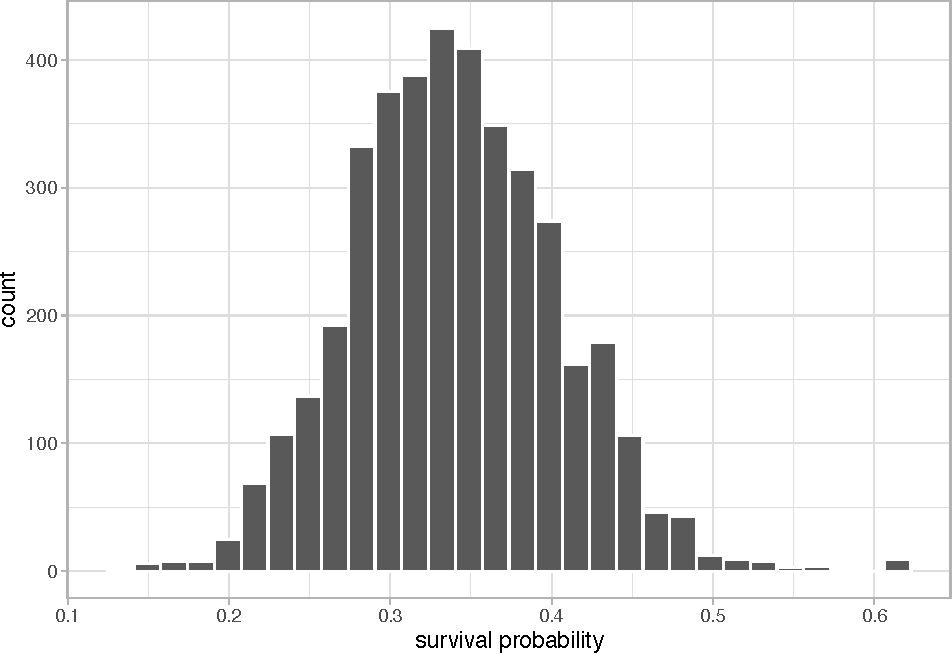
\includegraphics{banana-book_files/figure-latex/unnamed-chunk-41-1.pdf}

\hypertarget{post-process-mcmc-outputs-without-pain}{%
\subsection{Post-process MCMC outputs without pain}\label{post-process-mcmc-outputs-without-pain}}

We use MCMCvis, but there are other perfectly valid options out there like ggmcmc and basicMCMCplots.

Numerical summaries.

\begin{Shaded}
\begin{Highlighting}[]
\FunctionTok{library}\NormalTok{(MCMCvis)}
\FunctionTok{MCMCsummary}\NormalTok{(mcmc.output, }\AttributeTok{round =} \DecValTok{2}\NormalTok{)}
\DocumentationTok{\#\#       mean   sd 2.5\%  50\% 97.5\% Rhat n.eff}
\DocumentationTok{\#\# theta 0.34 0.06 0.22 0.34  0.47    1  1754}
\end{Highlighting}
\end{Shaded}

Trace and posterior density

\begin{Shaded}
\begin{Highlighting}[]
\FunctionTok{MCMCtrace}\NormalTok{(mcmc.output,}
          \AttributeTok{pdf =} \ConstantTok{FALSE}\NormalTok{)}
\end{Highlighting}
\end{Shaded}

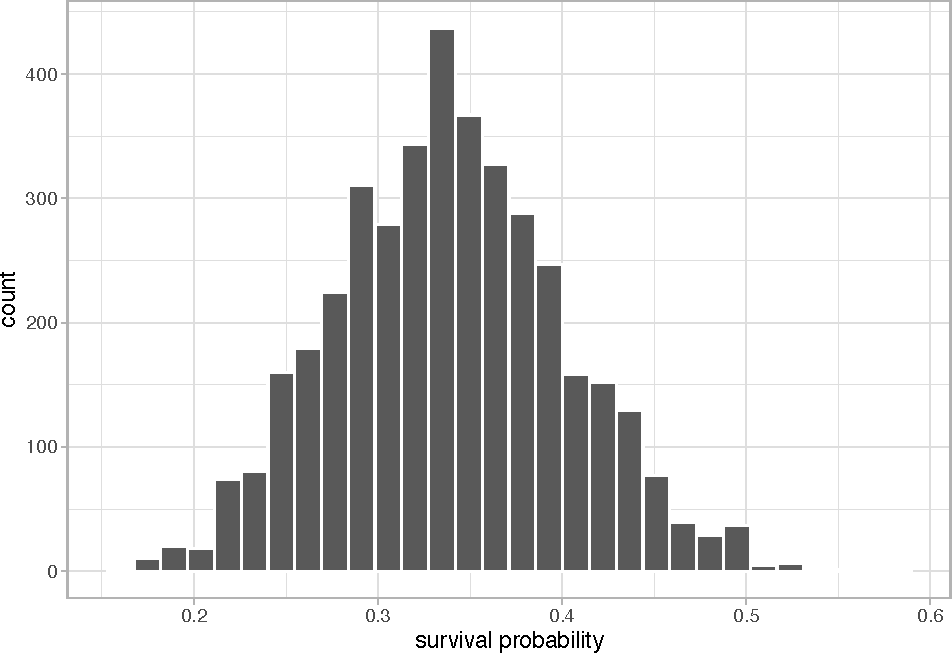
\includegraphics{banana-book_files/figure-latex/unnamed-chunk-43-1.pdf}

\begin{Shaded}
\begin{Highlighting}[]
\FunctionTok{MCMCtrace}\NormalTok{(mcmc.output,}
          \AttributeTok{pdf =} \ConstantTok{FALSE}\NormalTok{,}
          \AttributeTok{ind =} \ConstantTok{TRUE}\NormalTok{,}
          \AttributeTok{Rhat =} \ConstantTok{TRUE}\NormalTok{,}
          \AttributeTok{n.eff =} \ConstantTok{TRUE}\NormalTok{)}
\end{Highlighting}
\end{Shaded}

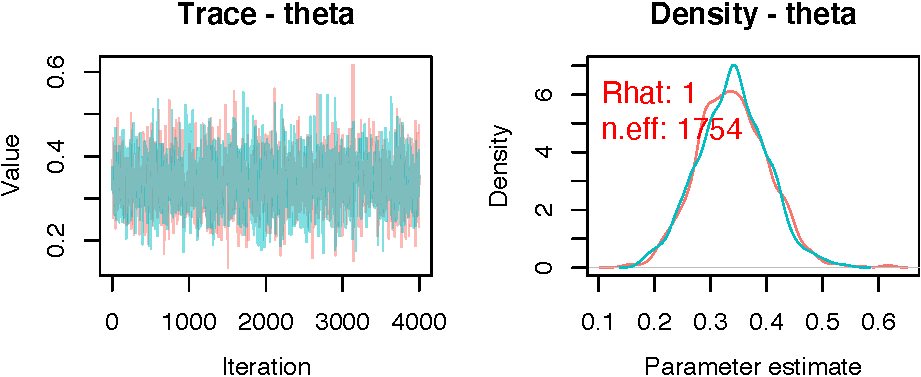
\includegraphics{banana-book_files/figure-latex/unnamed-chunk-44-1.pdf}

\hypertarget{syntax-whats-newbetterdifferent}{%
\section{Syntax: what's new/better/different?}\label{syntax-whats-newbetterdifferent}}

\textbf{basculer des trucs de speed up ici}

\begin{itemize}
\tightlist
\item
  Vectorization
\end{itemize}

\begin{Shaded}
\begin{Highlighting}[]
\CommentTok{\# JAGS (\& Nimble)}
\ControlFlowTok{for}\NormalTok{(t }\ControlFlowTok{in} \DecValTok{1}\SpecialCharTok{:}\NormalTok{Tmax)\{}
\NormalTok{  x[t] }\OtherTok{\textless{}{-}}\NormalTok{ Mu.x }\SpecialCharTok{+}\NormalTok{ epsilon[t]}
\NormalTok{\}}

\CommentTok{\# Nimble}
\NormalTok{x[}\DecValTok{1}\SpecialCharTok{:}\NormalTok{Tmax] }\OtherTok{\textless{}{-}}\NormalTok{ Mu.x }\SpecialCharTok{+}\NormalTok{ epsilon[}\DecValTok{1}\SpecialCharTok{:}\NormalTok{Tmax]}
\end{Highlighting}
\end{Shaded}

\begin{itemize}
\tightlist
\item
  More flexible specification of distributions
\end{itemize}

\begin{Shaded}
\begin{Highlighting}[]
\CommentTok{\# JAGS (\& Nimble)}
\ControlFlowTok{for}\NormalTok{(t }\ControlFlowTok{in} \DecValTok{1}\SpecialCharTok{:}\NormalTok{Tmax)\{}
\NormalTok{  epsilon[t] }\SpecialCharTok{\textasciitilde{}} \FunctionTok{dnorm}\NormalTok{(}\DecValTok{0}\NormalTok{, tau)}
\NormalTok{\}}
\NormalTok{tau }\OtherTok{\textless{}{-}} \FunctionTok{pow}\NormalTok{(sigma, }\SpecialCharTok{{-}}\DecValTok{2}\NormalTok{)}
\NormalTok{sigma }\SpecialCharTok{\textasciitilde{}} \FunctionTok{dunif}\NormalTok{(}\DecValTok{0}\NormalTok{, }\DecValTok{5}\NormalTok{)}

\CommentTok{\# Nimble}
\ControlFlowTok{for}\NormalTok{(t }\ControlFlowTok{in} \DecValTok{1}\SpecialCharTok{:}\NormalTok{Tmax)\{}
\NormalTok{  epsilon[t] }\SpecialCharTok{\textasciitilde{}} \FunctionTok{dnorm}\NormalTok{(}\DecValTok{0}\NormalTok{, }\AttributeTok{sd =}\NormalTok{ sigma)}
\NormalTok{\}}
\NormalTok{sigma }\SpecialCharTok{\textasciitilde{}} \FunctionTok{dunif}\NormalTok{(}\DecValTok{0}\NormalTok{, }\DecValTok{5}\NormalTok{)}
\end{Highlighting}
\end{Shaded}

\begin{itemize}
\tightlist
\item
  Your own functions and distributions
\end{itemize}

\begin{Shaded}
\begin{Highlighting}[]
\NormalTok{x[}\DecValTok{1}\SpecialCharTok{:}\NormalTok{Tmax] }\OtherTok{\textless{}{-}} \FunctionTok{myNimbleFunction}\NormalTok{(}\AttributeTok{a =}\NormalTok{ Mu.x, }\AttributeTok{b =}\NormalTok{ epsilon[}\DecValTok{1}\SpecialCharTok{:}\NormalTok{Tmax])}
\end{Highlighting}
\end{Shaded}

\begin{Shaded}
\begin{Highlighting}[]
\NormalTok{sigma }\SpecialCharTok{\textasciitilde{}} \FunctionTok{dCustomDistr}\NormalTok{(}\AttributeTok{c =} \FloatTok{0.5}\NormalTok{, }\AttributeTok{z =} \DecValTok{10}\NormalTok{)}
\end{Highlighting}
\end{Shaded}

\begin{itemize}
\tightlist
\item
  The end of empty indices
\end{itemize}

\begin{Shaded}
\begin{Highlighting}[]
\CommentTok{\# JAGS}
\NormalTok{sum.x }\OtherTok{\textless{}{-}} \FunctionTok{sum}\NormalTok{(x[])}

\CommentTok{\# Nimble}
\NormalTok{sum.x }\OtherTok{\textless{}{-}} \FunctionTok{sum}\NormalTok{(x[}\DecValTok{1}\SpecialCharTok{:}\NormalTok{Tmax])}
\end{Highlighting}
\end{Shaded}

\begin{itemize}
\tightlist
\item
  \& more\ldots{}
\end{itemize}

\hypertarget{our-nimble-workflow-so-far}{%
\section{\texorpdfstring{Our \texttt{nimble} workflow so far}{Our nimble workflow so far}}\label{our-nimble-workflow-so-far}}

\begin{Shaded}
\begin{Highlighting}[]
\NormalTok{knitr}\SpecialCharTok{::}\FunctionTok{include\_graphics}\NormalTok{(}\StringTok{"images/nimble\_workflow\_sofar.png"}\NormalTok{)}
\end{Highlighting}
\end{Shaded}

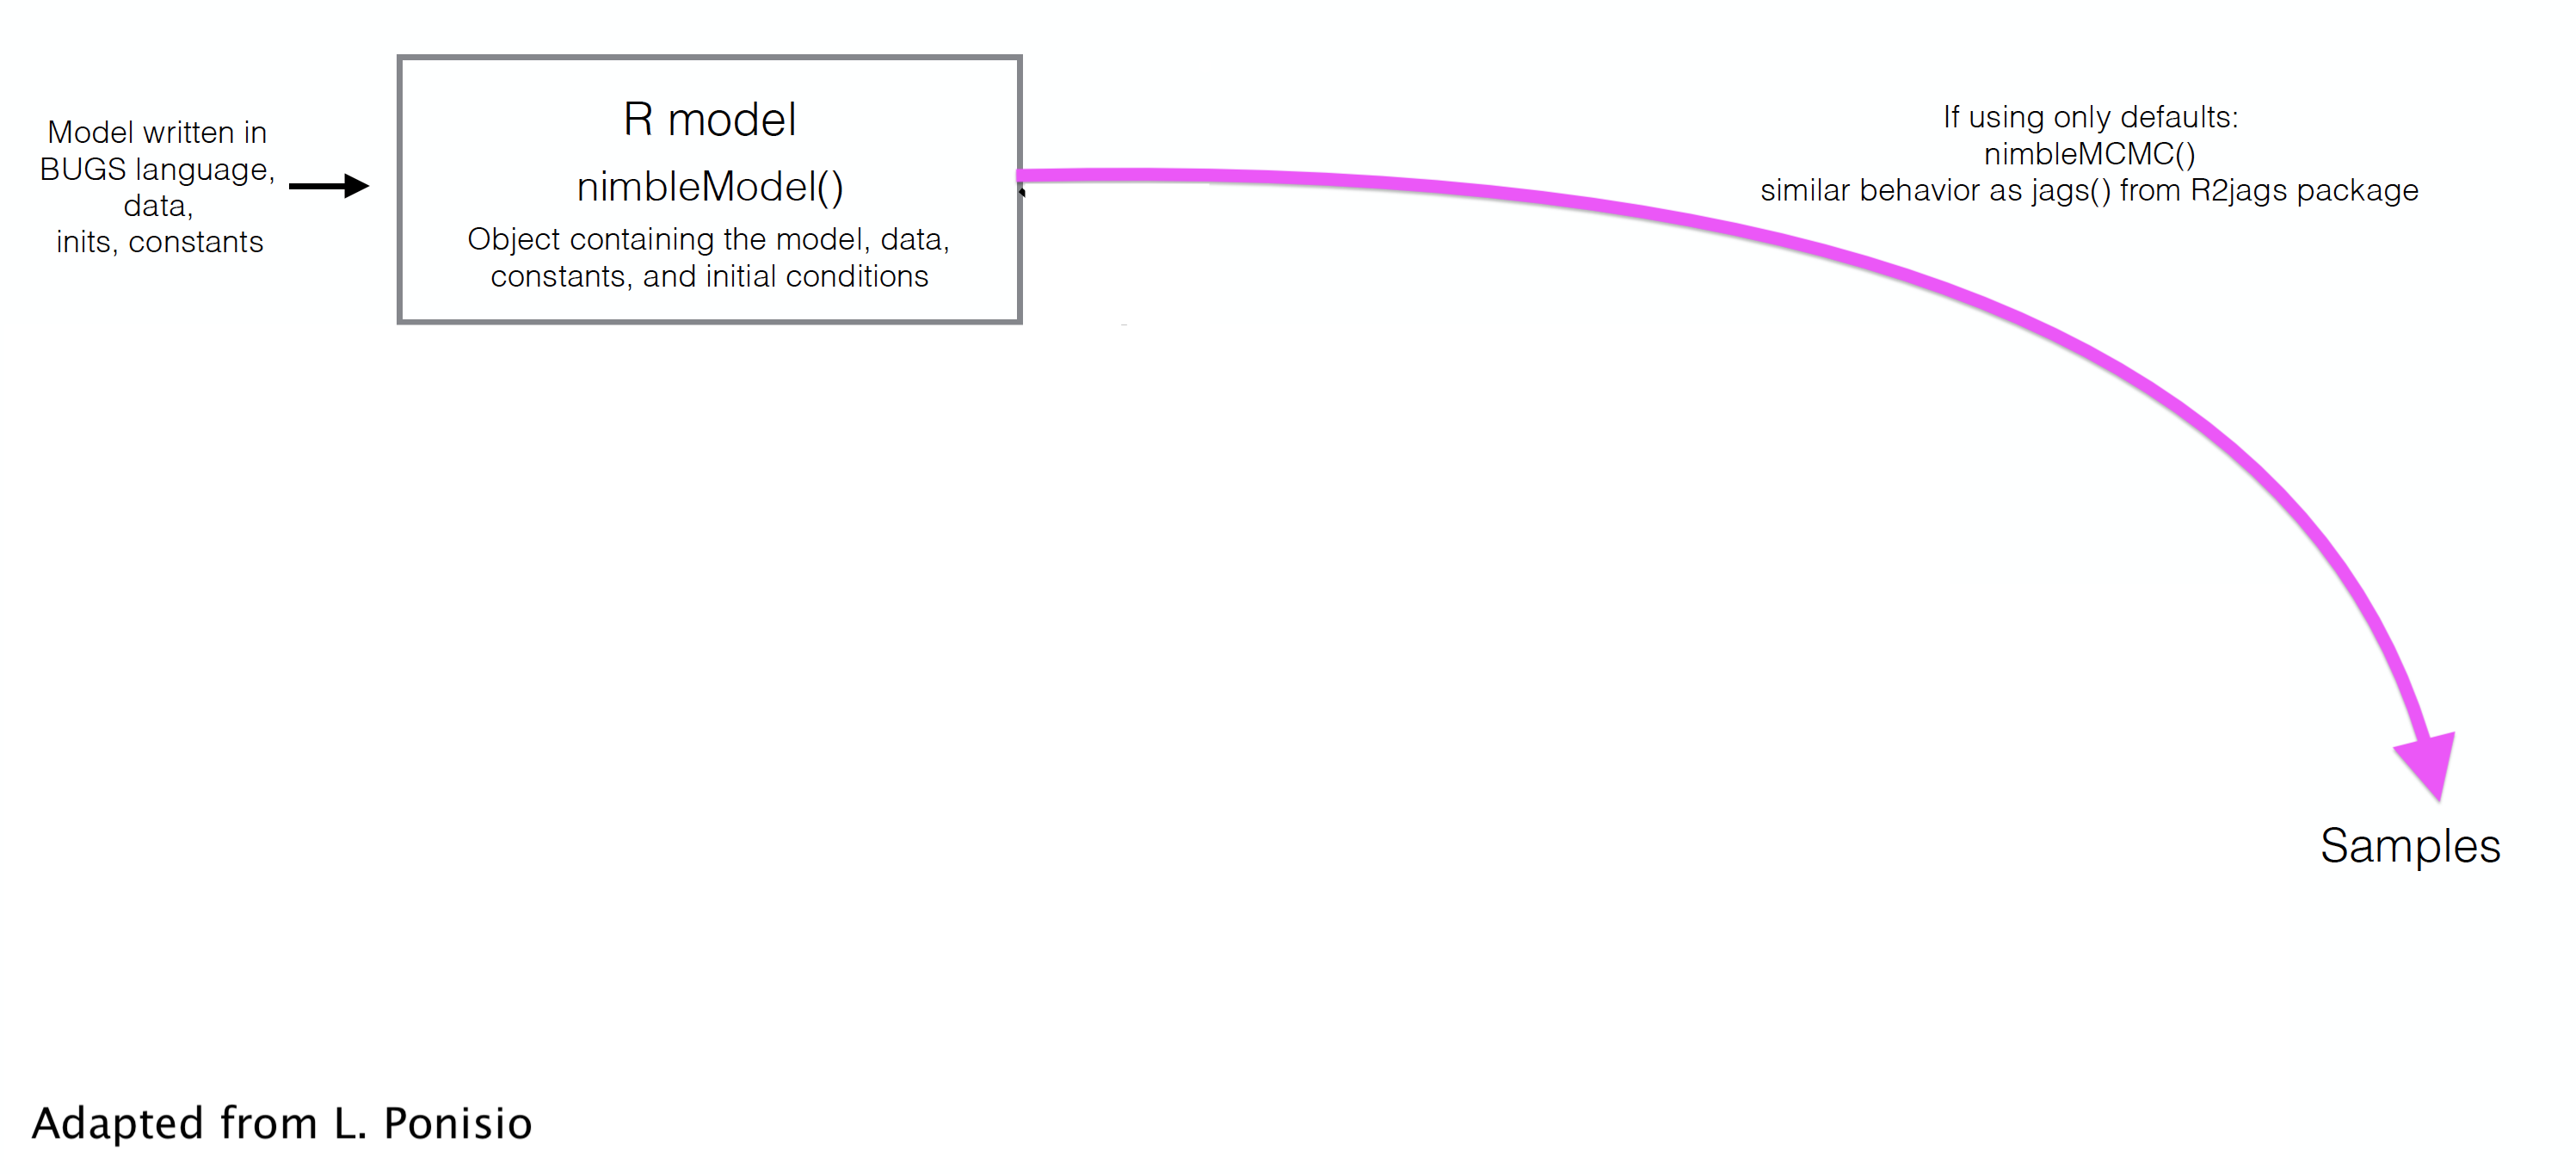
\includegraphics[width=41.58in]{images/nimble_workflow_sofar}

But \texttt{nimble} gives full access to the MCMC engine

\begin{Shaded}
\begin{Highlighting}[]
\NormalTok{knitr}\SpecialCharTok{::}\FunctionTok{include\_graphics}\NormalTok{(}\StringTok{"images/nimble\_workflow.png"}\NormalTok{)}
\end{Highlighting}
\end{Shaded}

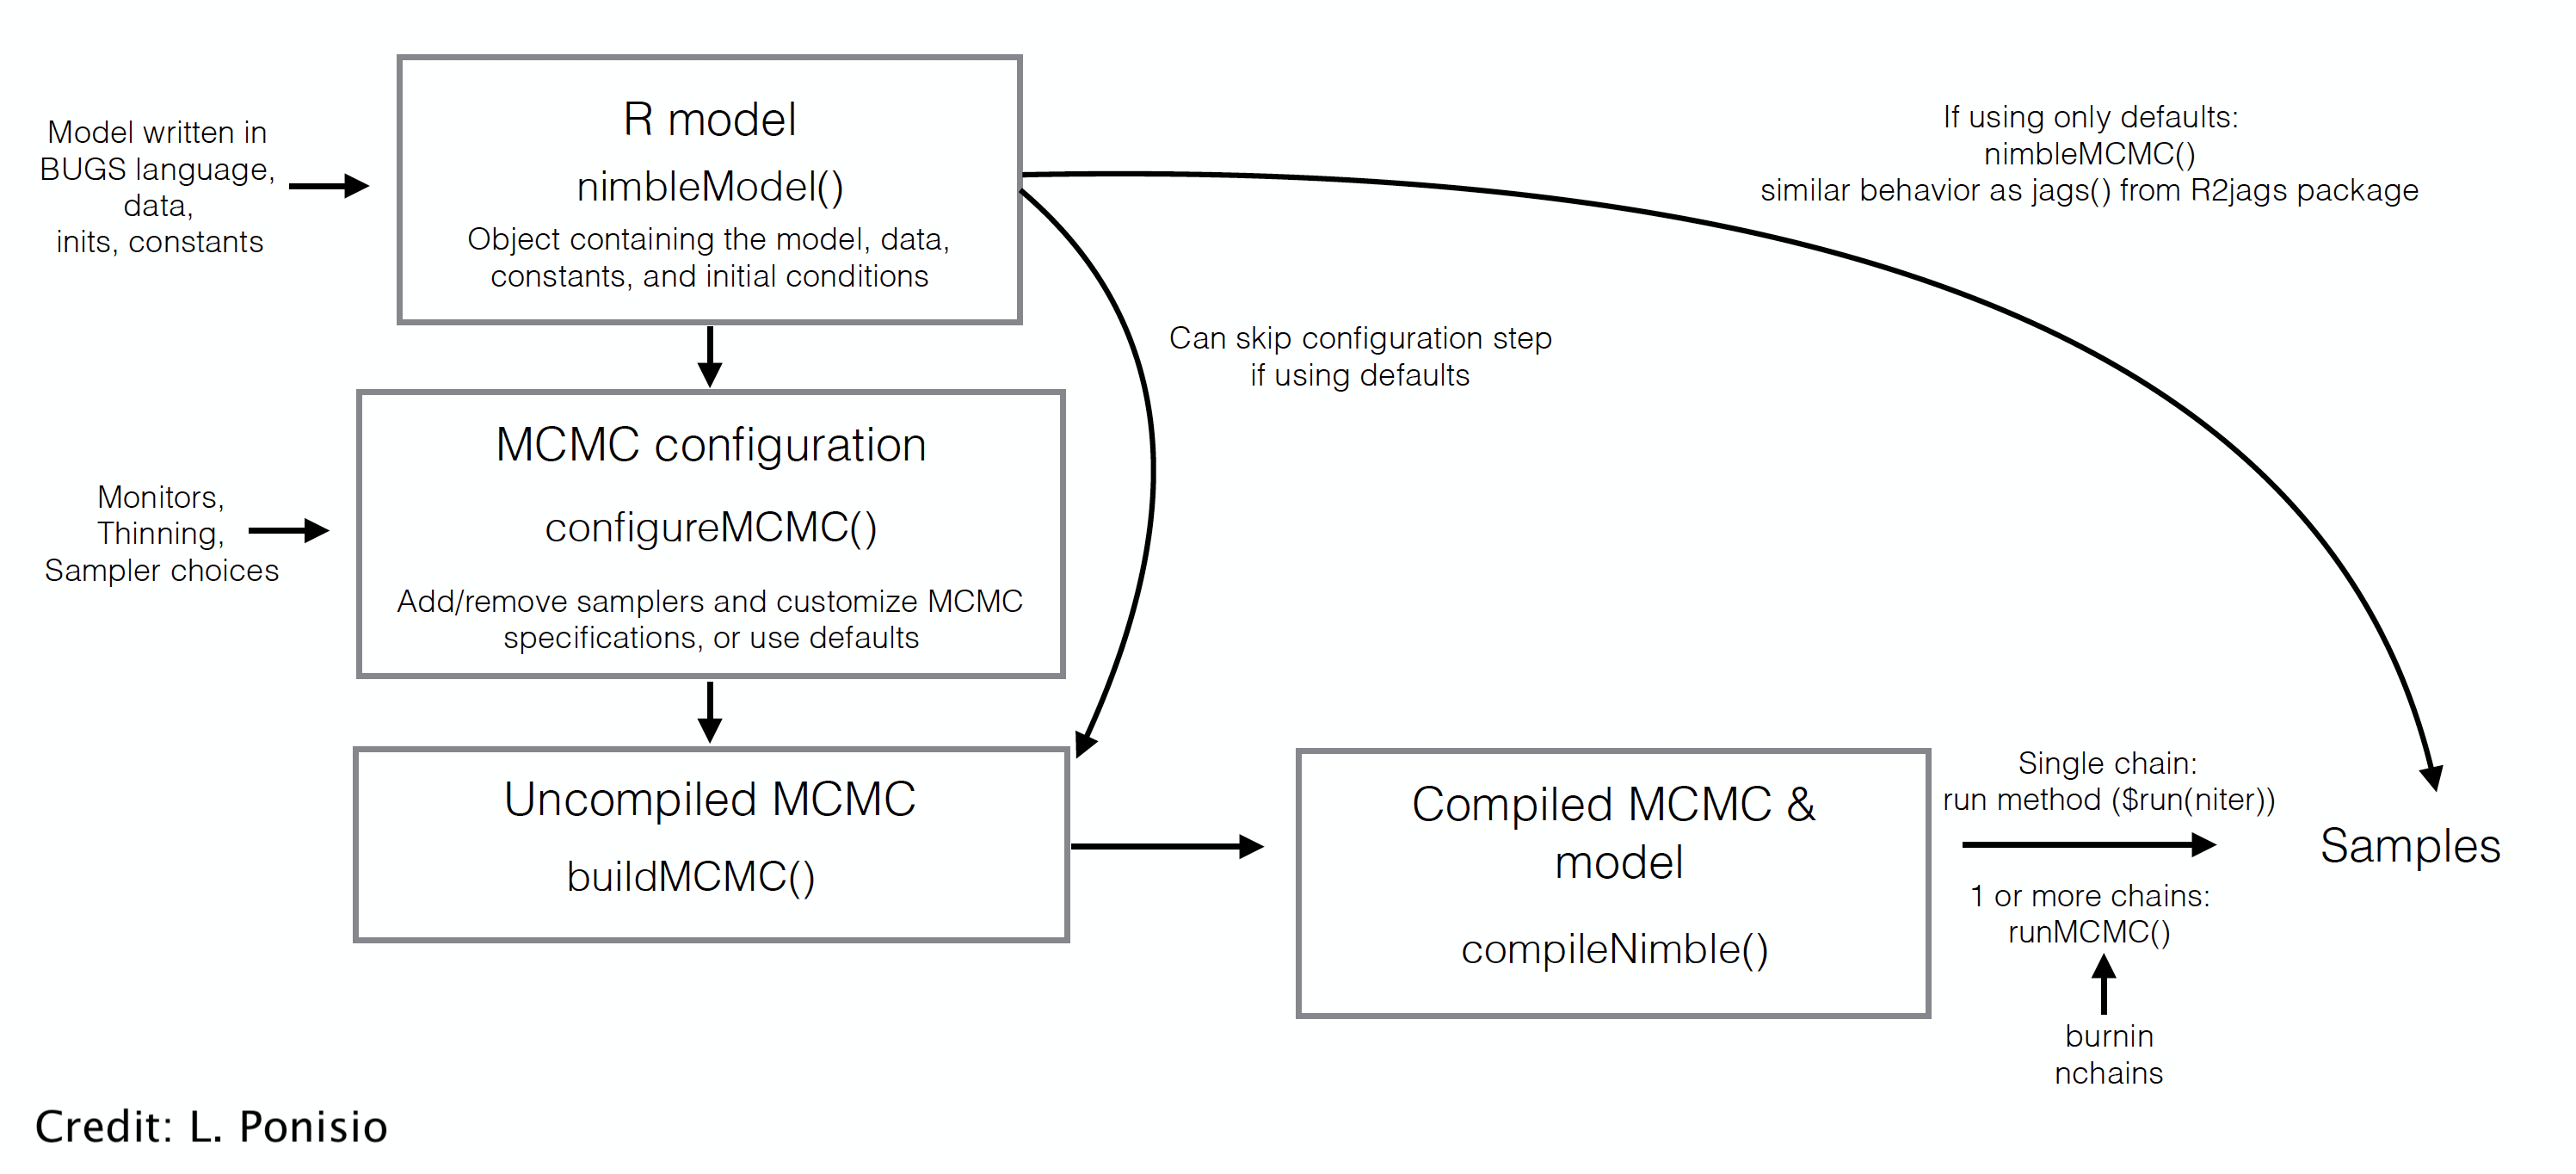
\includegraphics[width=41.58in]{images/nimble_workflow}

\begin{Shaded}
\begin{Highlighting}[]
\NormalTok{knitr}\SpecialCharTok{::}\FunctionTok{include\_graphics}\NormalTok{(}\StringTok{"images/I1bIY06.gif"}\NormalTok{)}
\end{Highlighting}
\end{Shaded}

\includegraphics{images/I1bIY06.gif}

\hypertarget{functions}{%
\section{Functions}\label{functions}}

Say we want an R function that adds 2 to every value in a vector.

\begin{Shaded}
\begin{Highlighting}[]
\NormalTok{add2 }\OtherTok{\textless{}{-}} \ControlFlowTok{function}\NormalTok{(x) \{}
\NormalTok{   x }\SpecialCharTok{+} \DecValTok{2} 
\NormalTok{\}}
\NormalTok{Radd2 }\OtherTok{\textless{}{-}} \FunctionTok{nimbleRcall}\NormalTok{(}\ControlFlowTok{function}\NormalTok{(}\AttributeTok{x =} \FunctionTok{double}\NormalTok{(}\DecValTok{0}\NormalTok{))\{\}, }
                     \AttributeTok{Rfun =} \StringTok{\textquotesingle{}add2\textquotesingle{}}\NormalTok{,}
                     \AttributeTok{returnType =} \FunctionTok{double}\NormalTok{(}\DecValTok{0}\NormalTok{))}
\NormalTok{demoCode }\OtherTok{\textless{}{-}} \FunctionTok{nimbleCode}\NormalTok{(\{}
\NormalTok{  mu }\SpecialCharTok{\textasciitilde{}} \FunctionTok{dnorm}\NormalTok{(}\DecValTok{0}\NormalTok{,}\DecValTok{1}\NormalTok{)}
  \ControlFlowTok{for}\NormalTok{(i }\ControlFlowTok{in} \DecValTok{1}\SpecialCharTok{:}\NormalTok{n) \{}
\NormalTok{    x[i] }\SpecialCharTok{\textasciitilde{}} \FunctionTok{dnorm}\NormalTok{(mu, }\AttributeTok{sd =} \DecValTok{1}\NormalTok{)}
\NormalTok{    z[i] }\OtherTok{\textless{}{-}} \FunctionTok{Radd2}\NormalTok{(x[i])}
\NormalTok{    \} }
\NormalTok{\})}

\NormalTok{param\_names }\OtherTok{\textless{}{-}} \FunctionTok{c}\NormalTok{(}\StringTok{"mu"}\NormalTok{, }\StringTok{"z"}\NormalTok{)}
\NormalTok{mcmc.out }\OtherTok{\textless{}{-}} \FunctionTok{nimbleMCMC}\NormalTok{(}\AttributeTok{code =}\NormalTok{ demoCode, }
                      \AttributeTok{constants =} \FunctionTok{list}\NormalTok{(}\AttributeTok{n =} \DecValTok{4}\NormalTok{),}
                      \AttributeTok{data =} \FunctionTok{list}\NormalTok{(}\AttributeTok{x =} \FunctionTok{c}\NormalTok{(}\SpecialCharTok{{-}}\DecValTok{1}\NormalTok{, }\SpecialCharTok{{-}}\DecValTok{2}\NormalTok{, }\DecValTok{1}\NormalTok{, }\DecValTok{2}\NormalTok{)), }
                      \AttributeTok{inits =} \FunctionTok{list}\NormalTok{(}\AttributeTok{mu =} \FunctionTok{rnorm}\NormalTok{(}\DecValTok{1}\NormalTok{)),}
                      \AttributeTok{monitors =}\NormalTok{ param\_names,}
                      \AttributeTok{nchains =} \DecValTok{2}\NormalTok{, }
                      \AttributeTok{niter =} \DecValTok{1000}\NormalTok{,}
                      \AttributeTok{nburnin =} \DecValTok{500}\NormalTok{)}
\DocumentationTok{\#\# |{-}{-}{-}{-}{-}{-}{-}{-}{-}{-}{-}{-}{-}|{-}{-}{-}{-}{-}{-}{-}{-}{-}{-}{-}{-}{-}|{-}{-}{-}{-}{-}{-}{-}{-}{-}{-}{-}{-}{-}|{-}{-}{-}{-}{-}{-}{-}{-}{-}{-}{-}{-}{-}|}
\DocumentationTok{\#\# |{-}{-}{-}{-}{-}{-}{-}{-}{-}{-}{-}{-}{-}{-}{-}{-}{-}{-}{-}{-}{-}{-}{-}{-}{-}{-}{-}{-}{-}{-}{-}{-}{-}{-}{-}{-}{-}{-}{-}{-}{-}{-}{-}{-}{-}{-}{-}{-}{-}{-}{-}{-}{-}{-}{-}|}
\DocumentationTok{\#\# |{-}{-}{-}{-}{-}{-}{-}{-}{-}{-}{-}{-}{-}|{-}{-}{-}{-}{-}{-}{-}{-}{-}{-}{-}{-}{-}|{-}{-}{-}{-}{-}{-}{-}{-}{-}{-}{-}{-}{-}|{-}{-}{-}{-}{-}{-}{-}{-}{-}{-}{-}{-}{-}|}
\DocumentationTok{\#\# |{-}{-}{-}{-}{-}{-}{-}{-}{-}{-}{-}{-}{-}{-}{-}{-}{-}{-}{-}{-}{-}{-}{-}{-}{-}{-}{-}{-}{-}{-}{-}{-}{-}{-}{-}{-}{-}{-}{-}{-}{-}{-}{-}{-}{-}{-}{-}{-}{-}{-}{-}{-}{-}{-}{-}|}
\FunctionTok{library}\NormalTok{(MCMCvis)}
\FunctionTok{MCMCsummary}\NormalTok{(}\AttributeTok{object =}\NormalTok{ mcmc.out, }\AttributeTok{round =} \DecValTok{2}\NormalTok{)}
\DocumentationTok{\#\#       mean   sd 2.5\% 50\% 97.5\% Rhat n.eff}
\DocumentationTok{\#\# mu   {-}0.01 0.46 {-}0.9   0  0.87    1   993}
\DocumentationTok{\#\# z[1]  1.00 0.00  1.0   1  1.00  NaN     0}
\DocumentationTok{\#\# z[2]  0.00 0.00  0.0   0  0.00  NaN     0}
\DocumentationTok{\#\# z[3]  3.00 0.00  3.0   3  3.00  NaN     0}
\DocumentationTok{\#\# z[4]  4.00 0.00  4.0   4  4.00  NaN     0}
\end{Highlighting}
\end{Shaded}

Change format to vectorise.

\begin{Shaded}
\begin{Highlighting}[]
\NormalTok{add2 }\OtherTok{\textless{}{-}} \ControlFlowTok{function}\NormalTok{(x) \{}
\NormalTok{   x }\SpecialCharTok{+} \DecValTok{2} 
\NormalTok{\}}
\NormalTok{Radd2 }\OtherTok{\textless{}{-}} \FunctionTok{nimbleRcall}\NormalTok{(}\ControlFlowTok{function}\NormalTok{(}\AttributeTok{x =} \FunctionTok{double}\NormalTok{(}\DecValTok{1}\NormalTok{))\{\}, }
                     \AttributeTok{Rfun =} \StringTok{\textquotesingle{}add2\textquotesingle{}}\NormalTok{,}
                     \AttributeTok{returnType =} \FunctionTok{double}\NormalTok{(}\DecValTok{1}\NormalTok{))}
\NormalTok{demoCode }\OtherTok{\textless{}{-}} \FunctionTok{nimbleCode}\NormalTok{(\{}
\NormalTok{  mu }\SpecialCharTok{\textasciitilde{}} \FunctionTok{dnorm}\NormalTok{(}\DecValTok{0}\NormalTok{,}\DecValTok{1}\NormalTok{)}
  \ControlFlowTok{for}\NormalTok{(i }\ControlFlowTok{in} \DecValTok{1}\SpecialCharTok{:}\NormalTok{n) \{}
\NormalTok{    x[i] }\SpecialCharTok{\textasciitilde{}} \FunctionTok{dnorm}\NormalTok{(mu, }\AttributeTok{sd =} \DecValTok{1}\NormalTok{)}
\NormalTok{    \}}
\NormalTok{    z[}\DecValTok{1}\SpecialCharTok{:}\DecValTok{4}\NormalTok{] }\OtherTok{\textless{}{-}} \FunctionTok{Radd2}\NormalTok{(x[}\DecValTok{1}\SpecialCharTok{:}\DecValTok{4}\NormalTok{])}
\NormalTok{\})}

\NormalTok{param\_names }\OtherTok{\textless{}{-}} \FunctionTok{c}\NormalTok{(}\StringTok{"mu"}\NormalTok{, }\StringTok{"z"}\NormalTok{)}
\NormalTok{mcmc.out }\OtherTok{\textless{}{-}} \FunctionTok{nimbleMCMC}\NormalTok{(}\AttributeTok{code =}\NormalTok{ demoCode, }
                      \AttributeTok{constants =} \FunctionTok{list}\NormalTok{(}\AttributeTok{n =} \DecValTok{4}\NormalTok{),}
                      \AttributeTok{data =} \FunctionTok{list}\NormalTok{(}\AttributeTok{x =} \FunctionTok{c}\NormalTok{(}\SpecialCharTok{{-}}\DecValTok{1}\NormalTok{, }\SpecialCharTok{{-}}\DecValTok{2}\NormalTok{, }\DecValTok{1}\NormalTok{, }\DecValTok{2}\NormalTok{)), }
                      \AttributeTok{inits =} \FunctionTok{list}\NormalTok{(}\AttributeTok{mu =} \FunctionTok{rnorm}\NormalTok{(}\DecValTok{1}\NormalTok{)),}
                      \AttributeTok{monitors =}\NormalTok{ param\_names,}
                      \AttributeTok{nchains =} \DecValTok{2}\NormalTok{, }
                      \AttributeTok{niter =} \DecValTok{1000}\NormalTok{,}
                      \AttributeTok{nburnin =} \DecValTok{500}\NormalTok{)}
\DocumentationTok{\#\# |{-}{-}{-}{-}{-}{-}{-}{-}{-}{-}{-}{-}{-}|{-}{-}{-}{-}{-}{-}{-}{-}{-}{-}{-}{-}{-}|{-}{-}{-}{-}{-}{-}{-}{-}{-}{-}{-}{-}{-}|{-}{-}{-}{-}{-}{-}{-}{-}{-}{-}{-}{-}{-}|}
\DocumentationTok{\#\# |{-}{-}{-}{-}{-}{-}{-}{-}{-}{-}{-}{-}{-}{-}{-}{-}{-}{-}{-}{-}{-}{-}{-}{-}{-}{-}{-}{-}{-}{-}{-}{-}{-}{-}{-}{-}{-}{-}{-}{-}{-}{-}{-}{-}{-}{-}{-}{-}{-}{-}{-}{-}{-}{-}{-}|}
\DocumentationTok{\#\# |{-}{-}{-}{-}{-}{-}{-}{-}{-}{-}{-}{-}{-}|{-}{-}{-}{-}{-}{-}{-}{-}{-}{-}{-}{-}{-}|{-}{-}{-}{-}{-}{-}{-}{-}{-}{-}{-}{-}{-}|{-}{-}{-}{-}{-}{-}{-}{-}{-}{-}{-}{-}{-}|}
\DocumentationTok{\#\# |{-}{-}{-}{-}{-}{-}{-}{-}{-}{-}{-}{-}{-}{-}{-}{-}{-}{-}{-}{-}{-}{-}{-}{-}{-}{-}{-}{-}{-}{-}{-}{-}{-}{-}{-}{-}{-}{-}{-}{-}{-}{-}{-}{-}{-}{-}{-}{-}{-}{-}{-}{-}{-}{-}{-}|}
\FunctionTok{library}\NormalTok{(MCMCvis)}
\FunctionTok{MCMCsummary}\NormalTok{(}\AttributeTok{object =}\NormalTok{ mcmc.out, }\AttributeTok{round =} \DecValTok{2}\NormalTok{)}
\DocumentationTok{\#\#      mean   sd  2.5\% 50\% 97.5\% Rhat n.eff}
\DocumentationTok{\#\# mu      0 0.45 {-}0.86   0  0.85    1  1150}
\DocumentationTok{\#\# z[1]    1 0.00  1.00   1  1.00  NaN     0}
\DocumentationTok{\#\# z[2]    0 0.00  0.00   0  0.00  NaN     0}
\DocumentationTok{\#\# z[3]    3 0.00  3.00   3  3.00  NaN     0}
\DocumentationTok{\#\# z[4]    4 0.00  4.00   4  4.00  NaN     0}
\end{Highlighting}
\end{Shaded}

Now have paramater to estimate as parameter of your R function.

\begin{Shaded}
\begin{Highlighting}[]
\NormalTok{add2 }\OtherTok{\textless{}{-}} \ControlFlowTok{function}\NormalTok{(x) \{}
\NormalTok{   x }\SpecialCharTok{+} \DecValTok{2} 
\NormalTok{\}}
\NormalTok{Radd2 }\OtherTok{\textless{}{-}} \FunctionTok{nimbleRcall}\NormalTok{(}\ControlFlowTok{function}\NormalTok{(}\AttributeTok{x =} \FunctionTok{double}\NormalTok{(}\DecValTok{0}\NormalTok{))\{\}, }
                     \AttributeTok{Rfun =} \StringTok{\textquotesingle{}add2\textquotesingle{}}\NormalTok{,}
                     \AttributeTok{returnType =} \FunctionTok{double}\NormalTok{(}\DecValTok{0}\NormalTok{))}
\NormalTok{demoCode }\OtherTok{\textless{}{-}} \FunctionTok{nimbleCode}\NormalTok{(\{}
\NormalTok{  mu }\SpecialCharTok{\textasciitilde{}} \FunctionTok{dnorm}\NormalTok{(}\DecValTok{0}\NormalTok{,}\DecValTok{1}\NormalTok{)}
  \ControlFlowTok{for}\NormalTok{(i }\ControlFlowTok{in} \DecValTok{1}\SpecialCharTok{:}\NormalTok{n) \{x[i] }\SpecialCharTok{\textasciitilde{}} \FunctionTok{dnorm}\NormalTok{(mu, }\AttributeTok{sd =} \DecValTok{1}\NormalTok{)\} }
\NormalTok{  z }\OtherTok{\textless{}{-}} \FunctionTok{Radd2}\NormalTok{(mu)}
\NormalTok{\})}

\NormalTok{param\_names }\OtherTok{\textless{}{-}} \FunctionTok{c}\NormalTok{(}\StringTok{"mu"}\NormalTok{, }\StringTok{"z"}\NormalTok{)}
\NormalTok{mcmc.out }\OtherTok{\textless{}{-}} \FunctionTok{nimbleMCMC}\NormalTok{(}\AttributeTok{code =}\NormalTok{ demoCode, }
                      \AttributeTok{constants =} \FunctionTok{list}\NormalTok{(}\AttributeTok{n =} \DecValTok{4}\NormalTok{),}
                      \AttributeTok{data =} \FunctionTok{list}\NormalTok{(}\AttributeTok{x =} \FunctionTok{c}\NormalTok{(}\SpecialCharTok{{-}}\DecValTok{1}\NormalTok{, }\SpecialCharTok{{-}}\DecValTok{2}\NormalTok{, }\DecValTok{1}\NormalTok{, }\DecValTok{2}\NormalTok{)), }
                      \AttributeTok{inits =} \FunctionTok{list}\NormalTok{(}\AttributeTok{mu =} \FunctionTok{rnorm}\NormalTok{(}\DecValTok{1}\NormalTok{)),}
                      \AttributeTok{monitors =}\NormalTok{ param\_names,}
                      \AttributeTok{nchains =} \DecValTok{2}\NormalTok{, }
                      \AttributeTok{niter =} \DecValTok{1000}\NormalTok{,}
                      \AttributeTok{nburnin =} \DecValTok{500}\NormalTok{)}
\DocumentationTok{\#\# |{-}{-}{-}{-}{-}{-}{-}{-}{-}{-}{-}{-}{-}|{-}{-}{-}{-}{-}{-}{-}{-}{-}{-}{-}{-}{-}|{-}{-}{-}{-}{-}{-}{-}{-}{-}{-}{-}{-}{-}|{-}{-}{-}{-}{-}{-}{-}{-}{-}{-}{-}{-}{-}|}
\DocumentationTok{\#\# |{-}{-}{-}{-}{-}{-}{-}{-}{-}{-}{-}{-}{-}{-}{-}{-}{-}{-}{-}{-}{-}{-}{-}{-}{-}{-}{-}{-}{-}{-}{-}{-}{-}{-}{-}{-}{-}{-}{-}{-}{-}{-}{-}{-}{-}{-}{-}{-}{-}{-}{-}{-}{-}{-}{-}|}
\DocumentationTok{\#\# |{-}{-}{-}{-}{-}{-}{-}{-}{-}{-}{-}{-}{-}|{-}{-}{-}{-}{-}{-}{-}{-}{-}{-}{-}{-}{-}|{-}{-}{-}{-}{-}{-}{-}{-}{-}{-}{-}{-}{-}|{-}{-}{-}{-}{-}{-}{-}{-}{-}{-}{-}{-}{-}|}
\DocumentationTok{\#\# |{-}{-}{-}{-}{-}{-}{-}{-}{-}{-}{-}{-}{-}{-}{-}{-}{-}{-}{-}{-}{-}{-}{-}{-}{-}{-}{-}{-}{-}{-}{-}{-}{-}{-}{-}{-}{-}{-}{-}{-}{-}{-}{-}{-}{-}{-}{-}{-}{-}{-}{-}{-}{-}{-}{-}|}
\FunctionTok{library}\NormalTok{(MCMCvis)}
\FunctionTok{MCMCsummary}\NormalTok{(}\AttributeTok{object =}\NormalTok{ mcmc.out, }\AttributeTok{round =} \DecValTok{2}\NormalTok{)}
\DocumentationTok{\#\#    mean   sd  2.5\% 50\% 97.5\% Rhat n.eff}
\DocumentationTok{\#\# mu    0 0.46 {-}0.92   0  0.87    1  1179}
\DocumentationTok{\#\# z     2 0.46  1.08   2  2.87    1  1179}
\end{Highlighting}
\end{Shaded}

In general if you do need a nimbleRcall like this, there are a couple of considerations. It is common to need to write a wrapper function, i.e.~a function you access via nimbleRcall that calls your actual function of interest with arguments and then return value rearranged as needed. For example, if you just need the eigenvectors, a wrapper function could pick those out and return them. The bigger issue is the returnType declaration: nimble type declarations do not include an R list of type declarations as a nimble type. I think you could use a nimbleList data structure for this purpose. You would have to create a nimbleList type and then use that as the declared returnType. But you would still need to write a wrapper, so that you could convert the list returned from base::eigen into a nimbleList object to return from your wrapper. I hope that makes sense.

\url{https://kenkellner.com/blog/models-with-integrals.html}

Same thing w/ global environment.

\begin{Shaded}
\begin{Highlighting}[]
\FunctionTok{library}\NormalTok{(nimble)}
\NormalTok{add2 }\OtherTok{\textless{}{-}} \ControlFlowTok{function}\NormalTok{(x) \{}
\NormalTok{   x }\SpecialCharTok{+} \DecValTok{2} \SpecialCharTok{+}\NormalTok{ globvar}
\NormalTok{\}}
\FunctionTok{add2}\NormalTok{(}\DecValTok{2}\NormalTok{)}
\NormalTok{globvar }\OtherTok{\textless{}{-}} \DecValTok{2020}
\FunctionTok{add2}\NormalTok{(}\DecValTok{2}\NormalTok{)}
\NormalTok{Radd2 }\OtherTok{\textless{}{-}} \FunctionTok{nimbleRcall}\NormalTok{(}\ControlFlowTok{function}\NormalTok{(}\AttributeTok{x =} \FunctionTok{double}\NormalTok{(}\DecValTok{0}\NormalTok{))\{\}, }
                     \AttributeTok{Rfun =} \StringTok{\textquotesingle{}add2\textquotesingle{}}\NormalTok{,}
                     \AttributeTok{returnType =} \FunctionTok{double}\NormalTok{(}\DecValTok{0}\NormalTok{))}
\NormalTok{demoCode }\OtherTok{\textless{}{-}} \FunctionTok{nimbleCode}\NormalTok{(\{}
\NormalTok{  mu }\SpecialCharTok{\textasciitilde{}} \FunctionTok{dnorm}\NormalTok{(}\DecValTok{0}\NormalTok{,}\DecValTok{1}\NormalTok{)}
  \ControlFlowTok{for}\NormalTok{(i }\ControlFlowTok{in} \DecValTok{1}\SpecialCharTok{:}\NormalTok{n) \{x[i] }\SpecialCharTok{\textasciitilde{}} \FunctionTok{dnorm}\NormalTok{(mu, }\AttributeTok{sd =} \DecValTok{1}\NormalTok{)\} }
\NormalTok{  z }\OtherTok{\textless{}{-}} \FunctionTok{Radd2}\NormalTok{(mu)}
\NormalTok{\})}

\NormalTok{param\_names }\OtherTok{\textless{}{-}} \FunctionTok{c}\NormalTok{(}\StringTok{"mu"}\NormalTok{, }\StringTok{"z"}\NormalTok{)}
\NormalTok{mcmc.out }\OtherTok{\textless{}{-}} \FunctionTok{nimbleMCMC}\NormalTok{(}\AttributeTok{code =}\NormalTok{ demoCode, }
                       \AttributeTok{constants =} \FunctionTok{list}\NormalTok{(}\AttributeTok{n =} \DecValTok{4}\NormalTok{),}
                       \AttributeTok{data =} \FunctionTok{list}\NormalTok{(}\AttributeTok{x =} \FunctionTok{c}\NormalTok{(}\SpecialCharTok{{-}}\DecValTok{1}\NormalTok{, }\SpecialCharTok{{-}}\DecValTok{2}\NormalTok{, }\DecValTok{1}\NormalTok{, }\DecValTok{2}\NormalTok{)), }
                       \AttributeTok{inits =} \FunctionTok{list}\NormalTok{(}\AttributeTok{mu =} \FunctionTok{rnorm}\NormalTok{(}\DecValTok{1}\NormalTok{)),}
                       \AttributeTok{monitors =}\NormalTok{ param\_names,}
                       \AttributeTok{nchains =} \DecValTok{2}\NormalTok{, }
                       \AttributeTok{niter =} \DecValTok{1000}\NormalTok{,}
                       \AttributeTok{nburnin =} \DecValTok{500}\NormalTok{)}
\CommentTok{\#printErrors()}
\CommentTok{\# pb is y is not recognized}
\CommentTok{\#ls()}
\CommentTok{\# assign y to global env}
\CommentTok{\# https://stackoverflow.com/questions/9726705/assign{-}multiple{-}objects{-}to{-}globalenv{-}from{-}within{-}a{-}function}
\CommentTok{\#assign("globvar", 20, envir = .GlobalEnv)}

\FunctionTok{library}\NormalTok{(MCMCvis)}
\FunctionTok{MCMCsummary}\NormalTok{(}\AttributeTok{object =}\NormalTok{ mcmc.out, }\AttributeTok{round =} \DecValTok{2}\NormalTok{)}
\end{Highlighting}
\end{Shaded}

\hypertarget{code-your-own-sampler}{%
\section{Code your own sampler}\label{code-your-own-sampler}}

\begin{Shaded}
\begin{Highlighting}[]
\FunctionTok{library}\NormalTok{(nimble)}
\FunctionTok{load}\NormalTok{(}\StringTok{\textquotesingle{}matos/ressources{-}chapters/nimble/dipper\_data.Rdata\textquotesingle{}}\NormalTok{)}

\NormalTok{dipperCode }\OtherTok{\textless{}{-}} \FunctionTok{nimbleCode}\NormalTok{(\{}
\NormalTok{    logit.p }\SpecialCharTok{\textasciitilde{}} \FunctionTok{dnorm}\NormalTok{(}\DecValTok{0}\NormalTok{, }\FloatTok{0.001}\NormalTok{)}
\NormalTok{    logit.phi }\SpecialCharTok{\textasciitilde{}} \FunctionTok{dnorm}\NormalTok{(}\DecValTok{0}\NormalTok{, }\FloatTok{0.001}\NormalTok{)}
\NormalTok{    p }\OtherTok{\textless{}{-}} \FunctionTok{expit}\NormalTok{(logit.p)}
\NormalTok{    phi }\OtherTok{\textless{}{-}} \FunctionTok{expit}\NormalTok{(logit.phi)}
    \DocumentationTok{\#\#phi \textasciitilde{} dunif(0, 1)}
    \DocumentationTok{\#\#p \textasciitilde{} dunif(0, 1)}
    \ControlFlowTok{for}\NormalTok{(i }\ControlFlowTok{in} \DecValTok{1}\SpecialCharTok{:}\NormalTok{N) \{}
\NormalTok{        x[i, first[i]] }\OtherTok{\textless{}{-}} \DecValTok{1}
\NormalTok{        y[i, first[i]] }\OtherTok{\textless{}{-}} \DecValTok{1}
        \ControlFlowTok{for}\NormalTok{(t }\ControlFlowTok{in}\NormalTok{ (first[i]}\SpecialCharTok{+}\DecValTok{1}\NormalTok{)}\SpecialCharTok{:}\NormalTok{T) \{}
\NormalTok{            x[i, t] }\SpecialCharTok{\textasciitilde{}} \FunctionTok{dbern}\NormalTok{(phi }\SpecialCharTok{*}\NormalTok{ x[i, t}\DecValTok{{-}1}\NormalTok{])}
\NormalTok{            y[i, t] }\SpecialCharTok{\textasciitilde{}} \FunctionTok{dbern}\NormalTok{(p }\SpecialCharTok{*}\NormalTok{ x[i, t])}
\NormalTok{        \}}
\NormalTok{    \}}
\NormalTok{\})}

\NormalTok{N }\OtherTok{\textless{}{-}} \FunctionTok{dim}\NormalTok{(sightings)[}\DecValTok{1}\NormalTok{]}
\NormalTok{T }\OtherTok{\textless{}{-}} \FunctionTok{dim}\NormalTok{(sightings)[}\DecValTok{2}\NormalTok{]}
\NormalTok{dipperConsts }\OtherTok{\textless{}{-}} \FunctionTok{list}\NormalTok{(}\AttributeTok{N =}\NormalTok{ N, }\AttributeTok{T =}\NormalTok{ T, }\AttributeTok{first =}\NormalTok{ first)}
\NormalTok{dipperData }\OtherTok{\textless{}{-}} \FunctionTok{list}\NormalTok{(}\AttributeTok{y =}\NormalTok{ sightings)}
\NormalTok{xInit }\OtherTok{\textless{}{-}} \FunctionTok{ifelse}\NormalTok{(}\SpecialCharTok{!}\FunctionTok{is.na}\NormalTok{(sightings), }\DecValTok{1}\NormalTok{, }\DecValTok{0}\NormalTok{)}
\NormalTok{dipperInits }\OtherTok{\textless{}{-}} \FunctionTok{list}\NormalTok{(}\AttributeTok{logit.phi =} \DecValTok{0}\NormalTok{, }\AttributeTok{logit.p =} \DecValTok{0}\NormalTok{, }\AttributeTok{x =}\NormalTok{ xInit)}

\NormalTok{samples }\OtherTok{\textless{}{-}} \FunctionTok{nimbleMCMC}\NormalTok{(dipperCode, dipperConsts, dipperData, dipperInits,}
                      \AttributeTok{niter =} \DecValTok{10000}\NormalTok{, }\AttributeTok{nburnin =} \DecValTok{5000}\NormalTok{,}
                      \AttributeTok{monitors =} \FunctionTok{c}\NormalTok{(}\StringTok{\textquotesingle{}p\textquotesingle{}}\NormalTok{, }\StringTok{\textquotesingle{}phi\textquotesingle{}}\NormalTok{))}

\NormalTok{my\_MH }\OtherTok{\textless{}{-}} \FunctionTok{nimbleFunction}\NormalTok{(}
    \AttributeTok{name =} \StringTok{\textquotesingle{}my\_MH\textquotesingle{}}\NormalTok{,}
    \AttributeTok{contains =}\NormalTok{ sampler\_BASE,}
    \AttributeTok{setup =} \ControlFlowTok{function}\NormalTok{(model, mvSaved, target, control) \{}
\NormalTok{        calcNodes }\OtherTok{\textless{}{-}}\NormalTok{ model}\SpecialCharTok{$}\FunctionTok{getDependencies}\NormalTok{(target)}
\NormalTok{        scale }\OtherTok{\textless{}{-}}\NormalTok{ control}\SpecialCharTok{$}\NormalTok{scale}
\NormalTok{    \},}
    \AttributeTok{run =} \ControlFlowTok{function}\NormalTok{() \{}
\NormalTok{        initialLP }\OtherTok{\textless{}{-}}\NormalTok{ model}\SpecialCharTok{$}\FunctionTok{getLogProb}\NormalTok{(calcNodes)}
\NormalTok{        current }\OtherTok{\textless{}{-}}\NormalTok{ model[[target]]}
\NormalTok{        proposal }\OtherTok{\textless{}{-}} \FunctionTok{rnorm}\NormalTok{(}\DecValTok{1}\NormalTok{, current, scale)}
\NormalTok{        model[[target]] }\OtherTok{\textless{}\textless{}{-}}\NormalTok{ proposal}
\NormalTok{        proposalLP }\OtherTok{\textless{}{-}}\NormalTok{ model}\SpecialCharTok{$}\FunctionTok{calculate}\NormalTok{(calcNodes)}
\NormalTok{        lMHR }\OtherTok{\textless{}{-}}\NormalTok{ proposalLP }\SpecialCharTok{{-}}\NormalTok{ initialLP}
        \ControlFlowTok{if}\NormalTok{(}\FunctionTok{runif}\NormalTok{(}\DecValTok{1}\NormalTok{,}\DecValTok{0}\NormalTok{,}\DecValTok{1}\NormalTok{) }\SpecialCharTok{\textless{}} \FunctionTok{exp}\NormalTok{(lMHR)) \{}
            \DocumentationTok{\#\# accept}
            \FunctionTok{copy}\NormalTok{(}\AttributeTok{from =}\NormalTok{ model, }\AttributeTok{to =}\NormalTok{ mvSaved, }\AttributeTok{nodes =}\NormalTok{ calcNodes, }\AttributeTok{logProb =} \ConstantTok{TRUE}\NormalTok{, }\AttributeTok{row =} \DecValTok{1}\NormalTok{)}
\NormalTok{        \} }\ControlFlowTok{else}\NormalTok{ \{}
            \DocumentationTok{\#\# reject}
            \FunctionTok{copy}\NormalTok{(}\AttributeTok{from =}\NormalTok{ mvSaved, }\AttributeTok{to =}\NormalTok{ model, }\AttributeTok{nodes =}\NormalTok{ calcNodes, }\AttributeTok{logProb =} \ConstantTok{TRUE}\NormalTok{, }\AttributeTok{row =} \DecValTok{1}\NormalTok{)}
\NormalTok{        \}}
\NormalTok{    \},}
    \AttributeTok{methods =} \FunctionTok{list}\NormalTok{(}
        \AttributeTok{reset =} \ControlFlowTok{function}\NormalTok{() \{\}}
\NormalTok{    )}
\NormalTok{)}

\NormalTok{scale }\OtherTok{\textless{}{-}} \FloatTok{0.05}

\NormalTok{Rmodel }\OtherTok{\textless{}{-}} \FunctionTok{nimbleModel}\NormalTok{(dipperCode, dipperConsts, dipperData, dipperInits)}
\NormalTok{conf }\OtherTok{\textless{}{-}} \FunctionTok{configureMCMC}\NormalTok{(Rmodel, }\AttributeTok{monitors =} \FunctionTok{c}\NormalTok{(}\StringTok{\textquotesingle{}p\textquotesingle{}}\NormalTok{, }\StringTok{\textquotesingle{}phi\textquotesingle{}}\NormalTok{))}
\NormalTok{conf}\SpecialCharTok{$}\FunctionTok{printSamplers}\NormalTok{()}
\NormalTok{conf}\SpecialCharTok{$}\FunctionTok{printSamplers}\NormalTok{(}\AttributeTok{byType =} \ConstantTok{TRUE}\NormalTok{)}
\NormalTok{conf}\SpecialCharTok{$}\FunctionTok{removeSamplers}\NormalTok{(}\FunctionTok{c}\NormalTok{(}\StringTok{\textquotesingle{}logit.p\textquotesingle{}}\NormalTok{, }\StringTok{\textquotesingle{}logit.phi\textquotesingle{}}\NormalTok{))}
\NormalTok{conf}\SpecialCharTok{$}\FunctionTok{addSampler}\NormalTok{(}\AttributeTok{target =} \StringTok{\textquotesingle{}logit.p\textquotesingle{}}\NormalTok{, }\AttributeTok{type =} \StringTok{\textquotesingle{}my\_MH\textquotesingle{}}\NormalTok{, }\AttributeTok{control =} \FunctionTok{list}\NormalTok{(}\AttributeTok{scale =}\NormalTok{ scale))}
\NormalTok{conf}\SpecialCharTok{$}\FunctionTok{addSampler}\NormalTok{(}\AttributeTok{target =} \StringTok{\textquotesingle{}logit.phi\textquotesingle{}}\NormalTok{, }\AttributeTok{type =} \StringTok{\textquotesingle{}my\_MH\textquotesingle{}}\NormalTok{, }\AttributeTok{control =} \FunctionTok{list}\NormalTok{(}\AttributeTok{scale =}\NormalTok{ scale))}
\NormalTok{conf}\SpecialCharTok{$}\FunctionTok{printSamplers}\NormalTok{()}
\NormalTok{conf}\SpecialCharTok{$}\FunctionTok{printMonitors}\NormalTok{()}
\NormalTok{Rmcmc }\OtherTok{\textless{}{-}} \FunctionTok{buildMCMC}\NormalTok{(conf)}

\NormalTok{out }\OtherTok{\textless{}{-}} \FunctionTok{compileNimble}\NormalTok{(}\FunctionTok{list}\NormalTok{(}\AttributeTok{model=}\NormalTok{Rmodel, }\AttributeTok{mcmc=}\NormalTok{Rmcmc))}
\NormalTok{Cmcmc }\OtherTok{\textless{}{-}}\NormalTok{ out}\SpecialCharTok{$}\NormalTok{mcmc}

\NormalTok{samples2 }\OtherTok{\textless{}{-}} \FunctionTok{runMCMC}\NormalTok{(Cmcmc, }\AttributeTok{niter =} \DecValTok{10000}\NormalTok{, }\AttributeTok{nburnin =} \DecValTok{5000}\NormalTok{)}

\FunctionTok{samplesSummary}\NormalTok{(samples2)}

\NormalTok{basicMCMCplots}\SpecialCharTok{::}\FunctionTok{chainsPlot}\NormalTok{(samples2)}
\end{Highlighting}
\end{Shaded}

\hypertarget{a-dire-quelque-part}{%
\section{A dire quelque part?}\label{a-dire-quelque-part}}

Pourquoi Nimble plutôt que Stan? Syntaxe BUGS, also discrete latent states easier to deal with, no need to marginalise. In Stan you marginalise (ref forward to relevant section of the book), but difficult endeavour, and you do not need to do that with NIMBLE, it has algorithms that work fine with discrete latent states.

\hypertarget{when-things-go-wrong-tip-and-tricks}{%
\section{When things go wrong: Tip and tricks}\label{when-things-go-wrong-tip-and-tricks}}

\hypertarget{summary-1}{%
\section{Summary}\label{summary-1}}

\begin{itemize}
\item
  Blabla.
\item
  Reblabla.
\end{itemize}

\begin{rmdnote}
The \emph{hypothesis} is a working assumption about which you want to learn using \emph{data}. In capture--recapture analyses, the hypothesis might be a parameter like detection probability, or regression parameters in a relationship between survival probability and a covariate. Bayes' theorem tells us how to obtain the probability of a hypothesis given the data we have.
\end{rmdnote}

\hypertarget{suggested-reading-1}{%
\section{Suggested reading}\label{suggested-reading-1}}

\begin{itemize}
\item
  Official website \url{https://r-nimble.org}
\item
  User Manual \url{https://r-nimble.org/html_manual/cha-welcome-nimble.html} and \href{https://r-nimble.org/cheatsheets/NimbleCheatSheet.pdf}{cheatsheet}.
\item
  Users mailing list \url{https://groups.google.com/forum/\#!forum/nimble-users}
\item
  Training material \url{https://github.com/nimble-training}
\item
  Reference to cite when using nimble in a publication:
\end{itemize}

\begin{quote}
de Valpine, P., D. Turek, C. J. Paciorek, C. Anderson-Bergman, D. Temple Lang, and R. Bodik (2017). \href{https://arxiv.org/pdf/1505.05093.pdf}{Programming With Models: Writing Statistical Algorithms for General Model Structures With NIMBLE}. \emph{Journal of Computational and Graphical Statistics} \textbf{26} (2): 403--13.
\end{quote}

\hypertarget{hmmcapturerecapture}{%
\chapter{Hidden Markov models}\label{hmmcapturerecapture}}

--\textgreater{}
--\textgreater{}

--\textgreater{}
--\textgreater{}
--\textgreater{}
--\textgreater{}
--\textgreater{}

\hypertarget{part-ii.-transitions}{%
\part{II. Transitions}\label{part-ii.-transitions}}

\hypertarget{introduction-3}{%
\chapter*{Introduction}\label{introduction-3}}


\hypertarget{survival}{%
\chapter{Survival}\label{survival}}

--\textgreater{}
--\textgreater{}

--\textgreater{}

--\textgreater{}

--\textgreater{}

--\textgreater{}
--\textgreater{}
--\textgreater{}

--\textgreater{}

--\textgreater{}
--\textgreater{}
--\textgreater{}
--\textgreater{}

\hypertarget{covariates}{%
\chapter{Covariates}\label{covariates}}

\hypertarget{dispersal}{%
\chapter{Dispersal}\label{dispersal}}

\hypertarget{model-selection}{%
\chapter{Model selection and validation}\label{model-selection}}

\hypertarget{part-iii.-states}{%
\part{III. States}\label{part-iii.-states}}

\hypertarget{introduction-4}{%
\chapter*{Introduction}\label{introduction-4}}


\hypertarget{uncertainty}{%
\chapter{State uncertainty}\label{uncertainty}}

\hypertarget{hsmm}{%
\chapter{Hidden semi-Markov models}\label{hsmm}}

\hypertarget{part-iv.-case-studies}{%
\part{IV. Case studies}\label{part-iv.-case-studies}}

\hypertarget{introduction-5}{%
\chapter*{Introduction}\label{introduction-5}}


\hypertarget{tradeoffs}{%
\chapter{Life history theory}\label{tradeoffs}}

\hypertarget{tradeoffs-1}{%
\section{Tradeoffs}\label{tradeoffs-1}}

\citet{morano_life-history_2013}, \citet{shefferson_life_2003}, and \citet{cruz-flores_sex-specific_nodate}

\hypertarget{breeding-dynamics}{%
\section{Breeding dynamics}\label{breeding-dynamics}}

\citet{pradel_breeding_2012}, \citet{desprez_now_2011}, \citet{desprez_known_2013}, and \citet{pacoureau_population_2019}

\hypertarget{actuarial-senescence}{%
\section{Actuarial senescence}\label{actuarial-senescence}}

\citet{choquet_semi-markov_2011}, \citet{peron_evidence_2016}

\hypertarget{cause-specific-mortalities}{%
\section{Cause-specific mortalities}\label{cause-specific-mortalities}}

\citet{fernandez-chacon_causes_2016} and \citet{ruette_comparative_2015}

\hypertarget{disease-dynamics}{%
\section{Disease dynamics}\label{disease-dynamics}}

\citet{MarescotEtAl2018} and \citet{santoro_multi-event_2014}

\hypertarget{sex-uncertainty}{%
\section{Sex uncertainty}\label{sex-uncertainty}}

\citet{PradelEtAl2008} and \citet{genovart_exploiting_2012}

\hypertarget{abundance}{%
\chapter{Abundance}\label{abundance}}

\hypertarget{horvitz-thompson}{%
\section{Horvitz-Thompson}\label{horvitz-thompson}}

\citet{santostasi_use_2019}

\hypertarget{jolly-seber}{%
\section{Jolly-Seber}\label{jolly-seber}}

\hypertarget{robust-design}{%
\section{Robust design}\label{robust-design}}

\citet{karamanlidis_evidence_2015}, \citet{santostasi_robust_2016}, \citet{gibson_application_2018}, and \citet{rankin_full-capture_2016}

\hypertarget{stopover}{%
\chapter{Stopover duration}\label{stopover}}

\citet{guerin_advances_2017}

\hypertarget{individual-dependence}{%
\chapter{Individual dependence}\label{individual-dependence}}

\hypertarget{dependence-among-individuals}{%
\section{Dependence among individuals}\label{dependence-among-individuals}}

\citet{culina_multievent_2013} and \citet{cubaynes_modeling_2021}

\hypertarget{individual-heterogeneity}{%
\section{Individual heterogeneity}\label{individual-heterogeneity}}

\citet{cubaynes_importance_2010}, \citet{gimenez_individual_2010}, and \citet{turek_bayesian_2021}

\hypertarget{part-v.-conclusion}{%
\part{V. Conclusion}\label{part-v.-conclusion}}

\hypertarget{take-home-messages}{%
\chapter*{Take-home messages}\label{take-home-messages}}


--\textgreater{}
--\textgreater{}

--\textgreater{}

--\textgreater{}

--\textgreater{}

\hypertarget{faq}{%
\chapter*{FAQ}\label{faq}}


\backmatter

  \bibliography{book.bib}

\printindex

\end{document}
